\documentclass[twoside]{book}

% Packages required by doxygen
\usepackage{fixltx2e}
\usepackage{calc}
\usepackage{doxygen}
\usepackage[export]{adjustbox} % also loads graphicx
\usepackage{graphicx}
\usepackage[utf8]{inputenc}
\usepackage{makeidx}
\usepackage{multicol}
\usepackage{multirow}
\PassOptionsToPackage{warn}{textcomp}
\usepackage{textcomp}
\usepackage[nointegrals]{wasysym}
\usepackage[table]{xcolor}

% Font selection
\usepackage[T1]{fontenc}
\usepackage[scaled=.90]{helvet}
\usepackage{courier}
\usepackage{amssymb}
\usepackage{sectsty}
\renewcommand{\familydefault}{\sfdefault}
\allsectionsfont{%
  \fontseries{bc}\selectfont%
  \color{darkgray}%
}
\renewcommand{\DoxyLabelFont}{%
  \fontseries{bc}\selectfont%
  \color{darkgray}%
}
\newcommand{\+}{\discretionary{\mbox{\scriptsize$\hookleftarrow$}}{}{}}

% Page & text layout
\usepackage{geometry}
\geometry{%
  a4paper,%
  top=2.5cm,%
  bottom=2.5cm,%
  left=2.5cm,%
  right=2.5cm%
}
\tolerance=750
\hfuzz=15pt
\hbadness=750
\setlength{\emergencystretch}{15pt}
\setlength{\parindent}{0cm}
\setlength{\parskip}{3ex plus 2ex minus 2ex}
\makeatletter
\renewcommand{\paragraph}{%
  \@startsection{paragraph}{4}{0ex}{-1.0ex}{1.0ex}{%
    \normalfont\normalsize\bfseries\SS@parafont%
  }%
}
\renewcommand{\subparagraph}{%
  \@startsection{subparagraph}{5}{0ex}{-1.0ex}{1.0ex}{%
    \normalfont\normalsize\bfseries\SS@subparafont%
  }%
}
\makeatother

% Headers & footers
\usepackage{fancyhdr}
\pagestyle{fancyplain}
\fancyhead[LE]{\fancyplain{}{\bfseries\thepage}}
\fancyhead[CE]{\fancyplain{}{}}
\fancyhead[RE]{\fancyplain{}{\bfseries\leftmark}}
\fancyhead[LO]{\fancyplain{}{\bfseries\rightmark}}
\fancyhead[CO]{\fancyplain{}{}}
\fancyhead[RO]{\fancyplain{}{\bfseries\thepage}}
\fancyfoot[LE]{\fancyplain{}{}}
\fancyfoot[CE]{\fancyplain{}{}}
\fancyfoot[RE]{\fancyplain{}{\bfseries\scriptsize Generated by Doxygen }}
\fancyfoot[LO]{\fancyplain{}{\bfseries\scriptsize Generated by Doxygen }}
\fancyfoot[CO]{\fancyplain{}{}}
\fancyfoot[RO]{\fancyplain{}{}}
\renewcommand{\footrulewidth}{0.4pt}
\renewcommand{\chaptermark}[1]{%
  \markboth{#1}{}%
}
\renewcommand{\sectionmark}[1]{%
  \markright{\thesection\ #1}%
}

% Indices & bibliography
\usepackage{natbib}
\usepackage[titles]{tocloft}
\setcounter{tocdepth}{3}
\setcounter{secnumdepth}{5}
\makeindex

% Hyperlinks (required, but should be loaded last)
\usepackage{ifpdf}
\ifpdf
  \usepackage[pdftex,pagebackref=true]{hyperref}
\else
  \usepackage[ps2pdf,pagebackref=true]{hyperref}
\fi
\hypersetup{%
  colorlinks=true,%
  linkcolor=blue,%
  citecolor=blue,%
  unicode%
}

% Custom commands
\newcommand{\clearemptydoublepage}{%
  \newpage{\pagestyle{empty}\cleardoublepage}%
}

\usepackage{caption}
\captionsetup{labelsep=space,justification=centering,font={bf},singlelinecheck=off,skip=4pt,position=top}

%===== C O N T E N T S =====

\begin{document}

% Titlepage & ToC
\hypersetup{pageanchor=false,
             bookmarksnumbered=true,
             pdfencoding=unicode
            }
\pagenumbering{alph}
\begin{titlepage}
\vspace*{7cm}
\begin{center}%
{\Large ug-\/thesis }\\
\vspace*{1cm}
{\large Generated by Doxygen 1.8.13}\\
\end{center}
\end{titlepage}
\clearemptydoublepage
\pagenumbering{roman}
\tableofcontents
\clearemptydoublepage
\pagenumbering{arabic}
\hypersetup{pageanchor=true}

%--- Begin generated contents ---
\chapter{Class Index}
\section{Class List}
Here are the classes, structs, unions and interfaces with brief descriptions\+:\begin{DoxyCompactList}
\item\contentsline{section}{\hyperlink{structattribute__info}{attribute\+\_\+info} }{\pageref{structattribute__info}}{}
\item\contentsline{section}{\hyperlink{classBytesParser}{Bytes\+Parser} \\*This struct handles the byte-\/by-\/byte parsing of a byte array }{\pageref{classBytesParser}}{}
\item\contentsline{section}{\hyperlink{classClassFileImpl}{Class\+File\+Impl} \\*This class represents an entire Java class }{\pageref{classClassFileImpl}}{}
\item\contentsline{section}{\hyperlink{classClassReader}{Class\+Reader} }{\pageref{classClassReader}}{}
\item\contentsline{section}{\hyperlink{classClassWriter}{Class\+Writer} }{\pageref{classClassWriter}}{}
\item\contentsline{section}{\hyperlink{structCode__attribute}{Code\+\_\+attribute} }{\pageref{structCode__attribute}}{}
\item\contentsline{section}{\hyperlink{structCONSTANT__Class__info}{C\+O\+N\+S\+T\+A\+N\+T\+\_\+\+Class\+\_\+info} }{\pageref{structCONSTANT__Class__info}}{}
\item\contentsline{section}{\hyperlink{structCONSTANT__GenericMethodref__info}{C\+O\+N\+S\+T\+A\+N\+T\+\_\+\+Generic\+Methodref\+\_\+info} }{\pageref{structCONSTANT__GenericMethodref__info}}{}
\item\contentsline{section}{\hyperlink{structCONSTANT__NameAndType__info}{C\+O\+N\+S\+T\+A\+N\+T\+\_\+\+Name\+And\+Type\+\_\+info} }{\pageref{structCONSTANT__NameAndType__info}}{}
\item\contentsline{section}{\hyperlink{structcp__info}{cp\+\_\+info} }{\pageref{structcp__info}}{}
\item\contentsline{section}{\hyperlink{structDebugOstream}{Debug\+Ostream} }{\pageref{structDebugOstream}}{}
\item\contentsline{section}{\hyperlink{structCode__attribute_1_1exception}{Code\+\_\+attribute\+::exception} }{\pageref{structCode__attribute_1_1exception}}{}
\item\contentsline{section}{\hyperlink{structfield__info}{field\+\_\+info} }{\pageref{structfield__info}}{}
\item\contentsline{section}{\hyperlink{structinterface__info}{interface\+\_\+info} }{\pageref{structinterface__info}}{}
\item\contentsline{section}{\hyperlink{classMethod}{Method} \\*This represents a view into a method reference of a class file }{\pageref{classMethod}}{}
\item\contentsline{section}{\hyperlink{structmethod__info}{method\+\_\+info} }{\pageref{structmethod__info}}{}
\item\contentsline{section}{\hyperlink{classProject}{Project} \\*A \hyperlink{classProject}{Project} is a collection of class files, together with a main entry point }{\pageref{classProject}}{}
\end{DoxyCompactList}

\chapter{Class Documentation}
\hypertarget{structattribute__info}{}\section{attribute\+\_\+info Struct Reference}
\label{structattribute__info}\index{attribute\+\_\+info@{attribute\+\_\+info}}


Collaboration diagram for attribute\+\_\+info\+:
\nopagebreak
\begin{figure}[H]
\begin{center}
\leavevmode
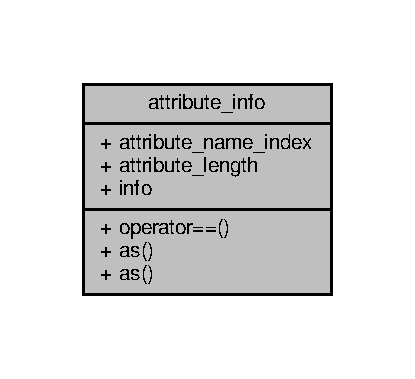
\includegraphics[width=199pt]{structattribute__info__coll__graph}
\end{center}
\end{figure}
\subsection*{Public Member Functions}
\begin{DoxyCompactItemize}
\item 
\mbox{\Hypertarget{structattribute__info_ace33b133435450d7d161751a3393de11}\label{structattribute__info_ace33b133435450d7d161751a3393de11}} 
{\footnotesize template$<$typename T $>$ }\\T \hyperlink{structattribute__info_ace33b133435450d7d161751a3393de11}{as} () const
\begin{DoxyCompactList}\small\item\em This template will be explicitly specialized for the possible types. \end{DoxyCompactList}\end{DoxyCompactItemize}


The documentation for this struct was generated from the following files\+:\begin{DoxyCompactItemize}
\item 
src/types.\+h\item 
src/types.\+cpp\end{DoxyCompactItemize}

\hypertarget{classBytesParser}{}\section{Bytes\+Parser Class Reference}
\label{classBytesParser}\index{Bytes\+Parser@{Bytes\+Parser}}


This struct handles the byte-\/by-\/byte parsing of a byte array.  




{\ttfamily \#include $<$bytesparser.\+h$>$}



Collaboration diagram for Bytes\+Parser\+:\nopagebreak
\begin{figure}[H]
\begin{center}
\leavevmode
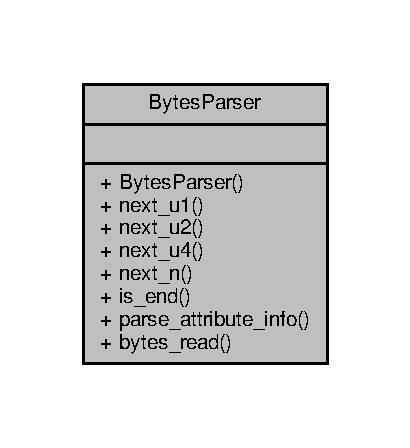
\includegraphics[width=197pt]{classBytesParser__coll__graph}
\end{center}
\end{figure}
\subsection*{Public Member Functions}
\begin{DoxyCompactItemize}
\item 
\hyperlink{classBytesParser_ac0b263b48e9a2be675442237cdc11f6c}{Bytes\+Parser} (std\+::vector$<$ \hyperlink{types_8h_a162f47a77ee24f6f77cd8c82ccd40ab7}{u1} $>$ data)
\item 
\hyperlink{types_8h_a162f47a77ee24f6f77cd8c82ccd40ab7}{u1} \hyperlink{classBytesParser_a18a5ff71458418a33c99d301ecc37579}{next\+\_\+u1} ()
\begin{DoxyCompactList}\small\item\em Consumes and returns the next unsigned char, in network order. \end{DoxyCompactList}\item 
\hyperlink{types_8h_ae676e9207f57fb921dca7366b2f59c53}{u2} \hyperlink{classBytesParser_a8c1d8a37eabff268351e38706a78ce2a}{next\+\_\+u2} ()
\begin{DoxyCompactList}\small\item\em Consumes and returns the next unsigned short, in network order. \end{DoxyCompactList}\item 
\hyperlink{types_8h_af3b2d4b29fd9faedc984db3e062b3d5d}{u4} \hyperlink{classBytesParser_a1023beb9a406a24c4080c95fbe8fd884}{next\+\_\+u4} ()
\begin{DoxyCompactList}\small\item\em Consumes and returns the next unsigned int, in network order. \end{DoxyCompactList}\item 
std\+::vector$<$ \hyperlink{types_8h_a162f47a77ee24f6f77cd8c82ccd40ab7}{u1} $>$ \hyperlink{classBytesParser_acb95ccefd93aa90ae9c74aaec13b497e}{next\+\_\+n} (int n)
\begin{DoxyCompactList}\small\item\em Consumes and returns the next {\ttfamily n} bytes. \end{DoxyCompactList}\item 
bool \hyperlink{classBytesParser_a0cef47c62af80c1a50fc507c5a869757}{is\+\_\+end} () const
\begin{DoxyCompactList}\small\item\em Returns whether all the data has been parsed. \end{DoxyCompactList}\item 
\hyperlink{structattribute__info}{attribute\+\_\+info} \hyperlink{classBytesParser_ab7c84f75bd3dc2bcac74fd3ff4c6510a}{parse\+\_\+attribute\+\_\+info} ()
\begin{DoxyCompactList}\small\item\em Parses an \hyperlink{structattribute__info}{attribute\+\_\+info} struct from the data buffer. \end{DoxyCompactList}\item 
int \hyperlink{classBytesParser_a37f2e2e19b23ba08982241c7ed53b43a}{bytes\+\_\+read} () const
\begin{DoxyCompactList}\small\item\em Returns how many bytes have been parsed so far. \end{DoxyCompactList}\end{DoxyCompactItemize}
\subsection*{Private Attributes}
\begin{DoxyCompactItemize}
\item 
std\+::vector$<$ \hyperlink{types_8h_a162f47a77ee24f6f77cd8c82ccd40ab7}{u1} $>$ \hyperlink{classBytesParser_a89b64c815664cea2869895e24d3e1ed3}{m\+\_\+data}
\item 
std\+::vector$<$ \hyperlink{types_8h_a162f47a77ee24f6f77cd8c82ccd40ab7}{u1} $>$\+::iterator \hyperlink{classBytesParser_a1116068a071fde3c2b634772c806af99}{m\+\_\+it}
\end{DoxyCompactItemize}


\subsection{Detailed Description}
This struct handles the byte-\/by-\/byte parsing of a byte array. 

\subsection{Constructor \& Destructor Documentation}
\mbox{\Hypertarget{classBytesParser_ac0b263b48e9a2be675442237cdc11f6c}\label{classBytesParser_ac0b263b48e9a2be675442237cdc11f6c}} 
\index{Bytes\+Parser@{Bytes\+Parser}!Bytes\+Parser@{Bytes\+Parser}}
\index{Bytes\+Parser@{Bytes\+Parser}!Bytes\+Parser@{Bytes\+Parser}}
\subsubsection{\texorpdfstring{Bytes\+Parser()}{BytesParser()}}
{\footnotesize\ttfamily Bytes\+Parser\+::\+Bytes\+Parser (\begin{DoxyParamCaption}\item[{std\+::vector$<$ \hyperlink{types_8h_a162f47a77ee24f6f77cd8c82ccd40ab7}{u1} $>$}]{data }\end{DoxyParamCaption})}



\subsection{Member Function Documentation}
\mbox{\Hypertarget{classBytesParser_a37f2e2e19b23ba08982241c7ed53b43a}\label{classBytesParser_a37f2e2e19b23ba08982241c7ed53b43a}} 
\index{Bytes\+Parser@{Bytes\+Parser}!bytes\+\_\+read@{bytes\+\_\+read}}
\index{bytes\+\_\+read@{bytes\+\_\+read}!Bytes\+Parser@{Bytes\+Parser}}
\subsubsection{\texorpdfstring{bytes\+\_\+read()}{bytes\_read()}}
{\footnotesize\ttfamily int Bytes\+Parser\+::bytes\+\_\+read (\begin{DoxyParamCaption}{ }\end{DoxyParamCaption}) const}



Returns how many bytes have been parsed so far. 

\mbox{\Hypertarget{classBytesParser_a0cef47c62af80c1a50fc507c5a869757}\label{classBytesParser_a0cef47c62af80c1a50fc507c5a869757}} 
\index{Bytes\+Parser@{Bytes\+Parser}!is\+\_\+end@{is\+\_\+end}}
\index{is\+\_\+end@{is\+\_\+end}!Bytes\+Parser@{Bytes\+Parser}}
\subsubsection{\texorpdfstring{is\+\_\+end()}{is\_end()}}
{\footnotesize\ttfamily bool Bytes\+Parser\+::is\+\_\+end (\begin{DoxyParamCaption}{ }\end{DoxyParamCaption}) const}



Returns whether all the data has been parsed. 

\mbox{\Hypertarget{classBytesParser_acb95ccefd93aa90ae9c74aaec13b497e}\label{classBytesParser_acb95ccefd93aa90ae9c74aaec13b497e}} 
\index{Bytes\+Parser@{Bytes\+Parser}!next\+\_\+n@{next\+\_\+n}}
\index{next\+\_\+n@{next\+\_\+n}!Bytes\+Parser@{Bytes\+Parser}}
\subsubsection{\texorpdfstring{next\+\_\+n()}{next\_n()}}
{\footnotesize\ttfamily std\+::vector$<$ \hyperlink{types_8h_a162f47a77ee24f6f77cd8c82ccd40ab7}{u1} $>$ Bytes\+Parser\+::next\+\_\+n (\begin{DoxyParamCaption}\item[{int}]{n }\end{DoxyParamCaption})}



Consumes and returns the next {\ttfamily n} bytes. 

Here is the call graph for this function\+:\nopagebreak
\begin{figure}[H]
\begin{center}
\leavevmode
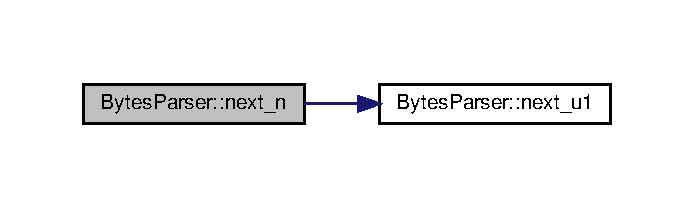
\includegraphics[width=333pt]{classBytesParser_acb95ccefd93aa90ae9c74aaec13b497e_cgraph}
\end{center}
\end{figure}
\mbox{\Hypertarget{classBytesParser_a18a5ff71458418a33c99d301ecc37579}\label{classBytesParser_a18a5ff71458418a33c99d301ecc37579}} 
\index{Bytes\+Parser@{Bytes\+Parser}!next\+\_\+u1@{next\+\_\+u1}}
\index{next\+\_\+u1@{next\+\_\+u1}!Bytes\+Parser@{Bytes\+Parser}}
\subsubsection{\texorpdfstring{next\+\_\+u1()}{next\_u1()}}
{\footnotesize\ttfamily \hyperlink{types_8h_a162f47a77ee24f6f77cd8c82ccd40ab7}{u1} Bytes\+Parser\+::next\+\_\+u1 (\begin{DoxyParamCaption}{ }\end{DoxyParamCaption})}



Consumes and returns the next unsigned char, in network order. 

\mbox{\Hypertarget{classBytesParser_a8c1d8a37eabff268351e38706a78ce2a}\label{classBytesParser_a8c1d8a37eabff268351e38706a78ce2a}} 
\index{Bytes\+Parser@{Bytes\+Parser}!next\+\_\+u2@{next\+\_\+u2}}
\index{next\+\_\+u2@{next\+\_\+u2}!Bytes\+Parser@{Bytes\+Parser}}
\subsubsection{\texorpdfstring{next\+\_\+u2()}{next\_u2()}}
{\footnotesize\ttfamily \hyperlink{types_8h_ae676e9207f57fb921dca7366b2f59c53}{u2} Bytes\+Parser\+::next\+\_\+u2 (\begin{DoxyParamCaption}{ }\end{DoxyParamCaption})}



Consumes and returns the next unsigned short, in network order. 

Here is the call graph for this function\+:\nopagebreak
\begin{figure}[H]
\begin{center}
\leavevmode
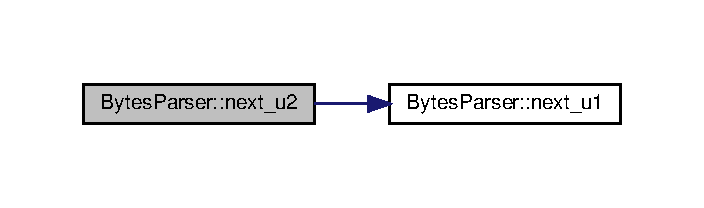
\includegraphics[width=338pt]{classBytesParser_a8c1d8a37eabff268351e38706a78ce2a_cgraph}
\end{center}
\end{figure}
\mbox{\Hypertarget{classBytesParser_a1023beb9a406a24c4080c95fbe8fd884}\label{classBytesParser_a1023beb9a406a24c4080c95fbe8fd884}} 
\index{Bytes\+Parser@{Bytes\+Parser}!next\+\_\+u4@{next\+\_\+u4}}
\index{next\+\_\+u4@{next\+\_\+u4}!Bytes\+Parser@{Bytes\+Parser}}
\subsubsection{\texorpdfstring{next\+\_\+u4()}{next\_u4()}}
{\footnotesize\ttfamily \hyperlink{types_8h_af3b2d4b29fd9faedc984db3e062b3d5d}{u4} Bytes\+Parser\+::next\+\_\+u4 (\begin{DoxyParamCaption}{ }\end{DoxyParamCaption})}



Consumes and returns the next unsigned int, in network order. 

Here is the call graph for this function\+:\nopagebreak
\begin{figure}[H]
\begin{center}
\leavevmode
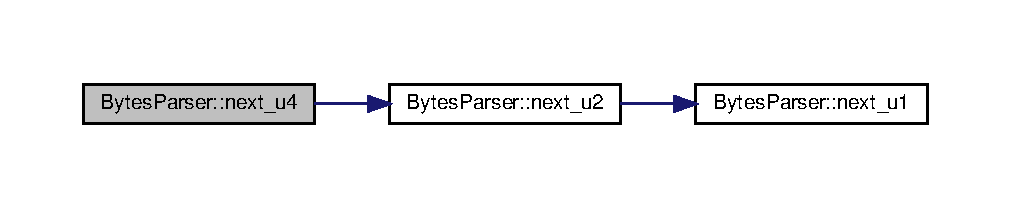
\includegraphics[width=350pt]{classBytesParser_a1023beb9a406a24c4080c95fbe8fd884_cgraph}
\end{center}
\end{figure}
\mbox{\Hypertarget{classBytesParser_ab7c84f75bd3dc2bcac74fd3ff4c6510a}\label{classBytesParser_ab7c84f75bd3dc2bcac74fd3ff4c6510a}} 
\index{Bytes\+Parser@{Bytes\+Parser}!parse\+\_\+attribute\+\_\+info@{parse\+\_\+attribute\+\_\+info}}
\index{parse\+\_\+attribute\+\_\+info@{parse\+\_\+attribute\+\_\+info}!Bytes\+Parser@{Bytes\+Parser}}
\subsubsection{\texorpdfstring{parse\+\_\+attribute\+\_\+info()}{parse\_attribute\_info()}}
{\footnotesize\ttfamily \hyperlink{structattribute__info}{attribute\+\_\+info} Bytes\+Parser\+::parse\+\_\+attribute\+\_\+info (\begin{DoxyParamCaption}{ }\end{DoxyParamCaption})}



Parses an \hyperlink{structattribute__info}{attribute\+\_\+info} struct from the data buffer. 

Here is the call graph for this function\+:\nopagebreak
\begin{figure}[H]
\begin{center}
\leavevmode
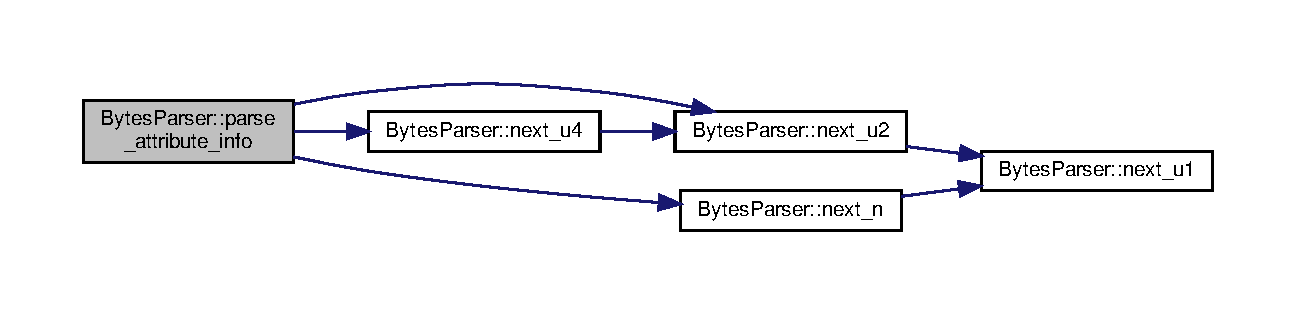
\includegraphics[width=350pt]{classBytesParser_ab7c84f75bd3dc2bcac74fd3ff4c6510a_cgraph}
\end{center}
\end{figure}


\subsection{Member Data Documentation}
\mbox{\Hypertarget{classBytesParser_a89b64c815664cea2869895e24d3e1ed3}\label{classBytesParser_a89b64c815664cea2869895e24d3e1ed3}} 
\index{Bytes\+Parser@{Bytes\+Parser}!m\+\_\+data@{m\+\_\+data}}
\index{m\+\_\+data@{m\+\_\+data}!Bytes\+Parser@{Bytes\+Parser}}
\subsubsection{\texorpdfstring{m\+\_\+data}{m\_data}}
{\footnotesize\ttfamily std\+::vector$<$\hyperlink{types_8h_a162f47a77ee24f6f77cd8c82ccd40ab7}{u1}$>$ Bytes\+Parser\+::m\+\_\+data\hspace{0.3cm}{\ttfamily [private]}}

\mbox{\Hypertarget{classBytesParser_a1116068a071fde3c2b634772c806af99}\label{classBytesParser_a1116068a071fde3c2b634772c806af99}} 
\index{Bytes\+Parser@{Bytes\+Parser}!m\+\_\+it@{m\+\_\+it}}
\index{m\+\_\+it@{m\+\_\+it}!Bytes\+Parser@{Bytes\+Parser}}
\subsubsection{\texorpdfstring{m\+\_\+it}{m\_it}}
{\footnotesize\ttfamily std\+::vector$<$\hyperlink{types_8h_a162f47a77ee24f6f77cd8c82ccd40ab7}{u1}$>$\+::iterator Bytes\+Parser\+::m\+\_\+it\hspace{0.3cm}{\ttfamily [private]}}



The documentation for this class was generated from the following files\+:\begin{DoxyCompactItemize}
\item 
src/\hyperlink{bytesparser_8h}{bytesparser.\+h}\item 
src/\hyperlink{bytesparser_8cpp}{bytesparser.\+cpp}\end{DoxyCompactItemize}

\hypertarget{classClassFileImpl}{}\section{Class\+File\+Impl Class Reference}
\label{classClassFileImpl}\index{Class\+File\+Impl@{Class\+File\+Impl}}


This class represents an entire Java class.  




{\ttfamily \#include $<$classfile.\+h$>$}



Collaboration diagram for Class\+File\+Impl\+:\nopagebreak
\begin{figure}[H]
\begin{center}
\leavevmode
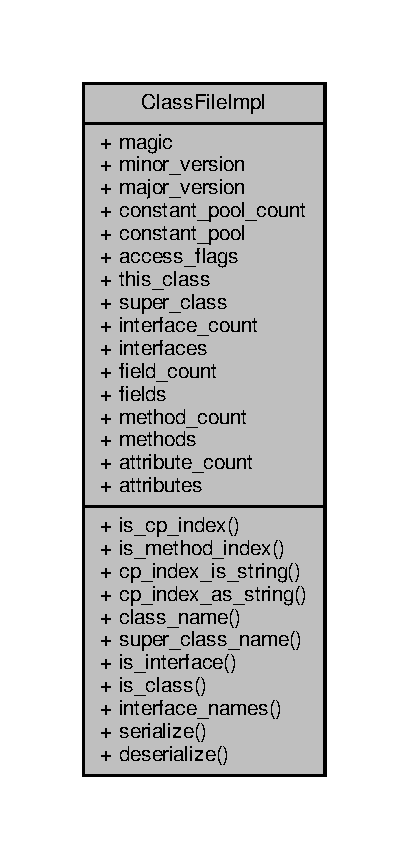
\includegraphics[width=196pt]{classClassFileImpl__coll__graph}
\end{center}
\end{figure}
\subsection*{Public Member Functions}
\begin{DoxyCompactItemize}
\item 
bool \hyperlink{classClassFileImpl_a1f15226f5107cb036e81d480531cda08}{is\+\_\+cp\+\_\+index} (int index) const
\item 
bool \hyperlink{classClassFileImpl_ad8f4fcb051aa9d8c04d67373abe12c43}{is\+\_\+method\+\_\+index} (int index) const
\begin{DoxyCompactList}\small\item\em Returns whether {\ttfamily index} is actually an index into the methods array. \end{DoxyCompactList}\item 
bool \hyperlink{classClassFileImpl_ab84cd50d25d163274a299ba682f57610}{cp\+\_\+index\+\_\+is\+\_\+string} (int index, const std\+::string \&s) const
\item 
std\+::string \hyperlink{classClassFileImpl_abf8923075c93d6d5bd1755a7b3ced362}{cp\+\_\+index\+\_\+as\+\_\+string} (int index) const
\item 
std\+::string \hyperlink{classClassFileImpl_a6b505e3750863370ca70c708d051a00c}{class\+\_\+name} () const
\begin{DoxyCompactList}\small\item\em Returns the name of the class corresponding to this classfile. \end{DoxyCompactList}\item 
std\+::string \hyperlink{classClassFileImpl_afd7229efcf341804086bcf6c00bb4820}{super\+\_\+class\+\_\+name} () const
\begin{DoxyCompactList}\small\item\em Returns the name of the super class. \end{DoxyCompactList}\item 
bool \hyperlink{classClassFileImpl_ade64e9cb17003aa71ef596785ab8c575}{is\+\_\+interface} () const
\begin{DoxyCompactList}\small\item\em Returns whether this is actually an interface, and not a class. \end{DoxyCompactList}\item 
bool \hyperlink{classClassFileImpl_a3772a57b8eaadf252a9a9f36c063ab93}{is\+\_\+class} () const
\item 
std\+::vector$<$ std\+::string $>$ \hyperlink{classClassFileImpl_ad2154cb52119b87cd74b722b69730dee}{interface\+\_\+names} () const
\item 
std\+::vector$<$ uint8\+\_\+t $>$ \hyperlink{classClassFileImpl_a4e2a4657d4b102369ba7305251d41d00}{serialize} () const
\begin{DoxyCompactList}\small\item\em Serialize the class file into binary data. \end{DoxyCompactList}\end{DoxyCompactItemize}
\subsection*{Static Public Member Functions}
\begin{DoxyCompactItemize}
\item 
static \hyperlink{classClassFileImpl}{Class\+File\+Impl} \hyperlink{classClassFileImpl_abdfa46cef80b0ec30115f1c0c9bb1db6}{deserialize} (const std\+::vector$<$ uint8\+\_\+t $>$ \&data)
\begin{DoxyCompactList}\small\item\em Deserialize the binary data into a class file. \end{DoxyCompactList}\end{DoxyCompactItemize}
\subsection*{Public Attributes}
\begin{DoxyCompactItemize}
\item 
\hyperlink{types_8h_af3b2d4b29fd9faedc984db3e062b3d5d}{u4} \hyperlink{classClassFileImpl_a31b4b986030442ae22f0630532032ded}{magic}
\item 
\hyperlink{types_8h_ae676e9207f57fb921dca7366b2f59c53}{u2} \hyperlink{classClassFileImpl_abec30809bc428ce5e31eebcd60a166e1}{minor\+\_\+version}
\item 
\hyperlink{types_8h_ae676e9207f57fb921dca7366b2f59c53}{u2} \hyperlink{classClassFileImpl_ac48ee85570e9e8b06f7a568a4246c2da}{major\+\_\+version}
\item 
\hyperlink{types_8h_ae676e9207f57fb921dca7366b2f59c53}{u2} \hyperlink{classClassFileImpl_ad1cf3a358e54bf290b8602808f2d3a0b}{constant\+\_\+pool\+\_\+count}
\item 
std\+::vector$<$ \hyperlink{structcp__info}{cp\+\_\+info} $>$ \hyperlink{classClassFileImpl_ac3a364b19cfd1a647309dcf385e8d064}{constant\+\_\+pool}
\item 
\hyperlink{types_8h_ae676e9207f57fb921dca7366b2f59c53}{u2} \hyperlink{classClassFileImpl_ae7bcc5b644d2164290c53a8727d36fb0}{access\+\_\+flags}
\item 
\hyperlink{types_8h_ae676e9207f57fb921dca7366b2f59c53}{u2} \hyperlink{classClassFileImpl_a63d984dbdc45e796e6599e2c0b982f36}{this\+\_\+class}
\item 
\hyperlink{types_8h_ae676e9207f57fb921dca7366b2f59c53}{u2} \hyperlink{classClassFileImpl_aa85098174076217a362065cbf00d804b}{super\+\_\+class}
\item 
\hyperlink{types_8h_ae676e9207f57fb921dca7366b2f59c53}{u2} \hyperlink{classClassFileImpl_ae8948beaa9ebac1d5df2c73ec62602c8}{interface\+\_\+count}
\item 
std\+::vector$<$ \hyperlink{structinterface__info}{interface\+\_\+info} $>$ \hyperlink{classClassFileImpl_a449222435f48682e0f680432cf03f49b}{interfaces}
\item 
\hyperlink{types_8h_ae676e9207f57fb921dca7366b2f59c53}{u2} \hyperlink{classClassFileImpl_a0144ff86144e3548e32779faf4e0dab9}{field\+\_\+count}
\item 
std\+::vector$<$ \hyperlink{structfield__info}{field\+\_\+info} $>$ \hyperlink{classClassFileImpl_af0ba1073f7566cdb21c47d33198ecab0}{fields}
\item 
\hyperlink{types_8h_ae676e9207f57fb921dca7366b2f59c53}{u2} \hyperlink{classClassFileImpl_a9643bb90606a32fa3f4a35f2ff468e5b}{method\+\_\+count}
\item 
std\+::vector$<$ \hyperlink{structmethod__info}{method\+\_\+info} $>$ \hyperlink{classClassFileImpl_a9142d753fc1a3b06ce26606506b2e9c1}{methods}
\item 
\hyperlink{types_8h_ae676e9207f57fb921dca7366b2f59c53}{u2} \hyperlink{classClassFileImpl_ac1085cebfdbb8a2469d9de9782d0576d}{attribute\+\_\+count}
\item 
std\+::vector$<$ \hyperlink{structattribute__info}{attribute\+\_\+info} $>$ \hyperlink{classClassFileImpl_a25689268cd6201a1b970a6dd41ac6fce}{attributes}
\end{DoxyCompactItemize}


\subsection{Detailed Description}
This class represents an entire Java class. 

\subsection{Member Function Documentation}
\mbox{\Hypertarget{classClassFileImpl_a6b505e3750863370ca70c708d051a00c}\label{classClassFileImpl_a6b505e3750863370ca70c708d051a00c}} 
\index{Class\+File\+Impl@{Class\+File\+Impl}!class\+\_\+name@{class\+\_\+name}}
\index{class\+\_\+name@{class\+\_\+name}!Class\+File\+Impl@{Class\+File\+Impl}}
\subsubsection{\texorpdfstring{class\+\_\+name()}{class\_name()}}
{\footnotesize\ttfamily std\+::string Class\+File\+Impl\+::class\+\_\+name (\begin{DoxyParamCaption}{ }\end{DoxyParamCaption}) const}



Returns the name of the class corresponding to this classfile. 

Here is the call graph for this function\+:
\nopagebreak
\begin{figure}[H]
\begin{center}
\leavevmode
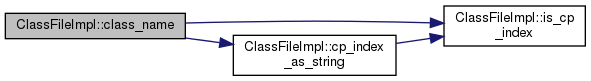
\includegraphics[width=350pt]{classClassFileImpl_a6b505e3750863370ca70c708d051a00c_cgraph}
\end{center}
\end{figure}
\mbox{\Hypertarget{classClassFileImpl_abf8923075c93d6d5bd1755a7b3ced362}\label{classClassFileImpl_abf8923075c93d6d5bd1755a7b3ced362}} 
\index{Class\+File\+Impl@{Class\+File\+Impl}!cp\+\_\+index\+\_\+as\+\_\+string@{cp\+\_\+index\+\_\+as\+\_\+string}}
\index{cp\+\_\+index\+\_\+as\+\_\+string@{cp\+\_\+index\+\_\+as\+\_\+string}!Class\+File\+Impl@{Class\+File\+Impl}}
\subsubsection{\texorpdfstring{cp\+\_\+index\+\_\+as\+\_\+string()}{cp\_index\_as\_string()}}
{\footnotesize\ttfamily std\+::string Class\+File\+Impl\+::cp\+\_\+index\+\_\+as\+\_\+string (\begin{DoxyParamCaption}\item[{int}]{index }\end{DoxyParamCaption}) const}

Asserts that the constant at index {\ttfamily index} is an utf8 string, and returns it. Here is the call graph for this function\+:
\nopagebreak
\begin{figure}[H]
\begin{center}
\leavevmode
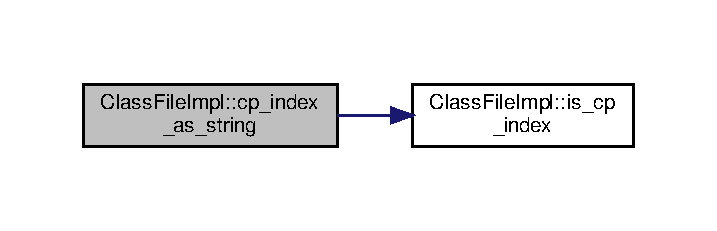
\includegraphics[width=344pt]{classClassFileImpl_abf8923075c93d6d5bd1755a7b3ced362_cgraph}
\end{center}
\end{figure}
\mbox{\Hypertarget{classClassFileImpl_ab84cd50d25d163274a299ba682f57610}\label{classClassFileImpl_ab84cd50d25d163274a299ba682f57610}} 
\index{Class\+File\+Impl@{Class\+File\+Impl}!cp\+\_\+index\+\_\+is\+\_\+string@{cp\+\_\+index\+\_\+is\+\_\+string}}
\index{cp\+\_\+index\+\_\+is\+\_\+string@{cp\+\_\+index\+\_\+is\+\_\+string}!Class\+File\+Impl@{Class\+File\+Impl}}
\subsubsection{\texorpdfstring{cp\+\_\+index\+\_\+is\+\_\+string()}{cp\_index\_is\_string()}}
{\footnotesize\ttfamily bool Class\+File\+Impl\+::cp\+\_\+index\+\_\+is\+\_\+string (\begin{DoxyParamCaption}\item[{int}]{index,  }\item[{const std\+::string \&}]{s }\end{DoxyParamCaption}) const}

Returns whether the index {\ttfamily index} is a string, and corresponds to the string {\ttfamily s}. Note that this asserts that the index is actually contained within the constant pool. Here is the call graph for this function\+:
\nopagebreak
\begin{figure}[H]
\begin{center}
\leavevmode
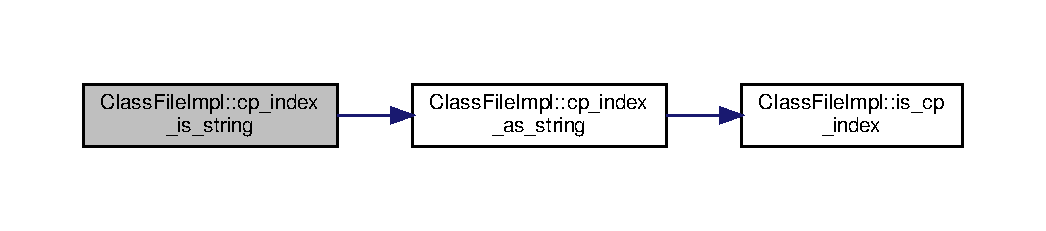
\includegraphics[width=350pt]{classClassFileImpl_ab84cd50d25d163274a299ba682f57610_cgraph}
\end{center}
\end{figure}
\mbox{\Hypertarget{classClassFileImpl_abdfa46cef80b0ec30115f1c0c9bb1db6}\label{classClassFileImpl_abdfa46cef80b0ec30115f1c0c9bb1db6}} 
\index{Class\+File\+Impl@{Class\+File\+Impl}!deserialize@{deserialize}}
\index{deserialize@{deserialize}!Class\+File\+Impl@{Class\+File\+Impl}}
\subsubsection{\texorpdfstring{deserialize()}{deserialize()}}
{\footnotesize\ttfamily \hyperlink{classClassFileImpl}{Class\+File\+Impl} Class\+File\+Impl\+::deserialize (\begin{DoxyParamCaption}\item[{const std\+::vector$<$ uint8\+\_\+t $>$ \&}]{data }\end{DoxyParamCaption})\hspace{0.3cm}{\ttfamily [static]}}



Deserialize the binary data into a class file. 

Here is the call graph for this function\+:
\nopagebreak
\begin{figure}[H]
\begin{center}
\leavevmode
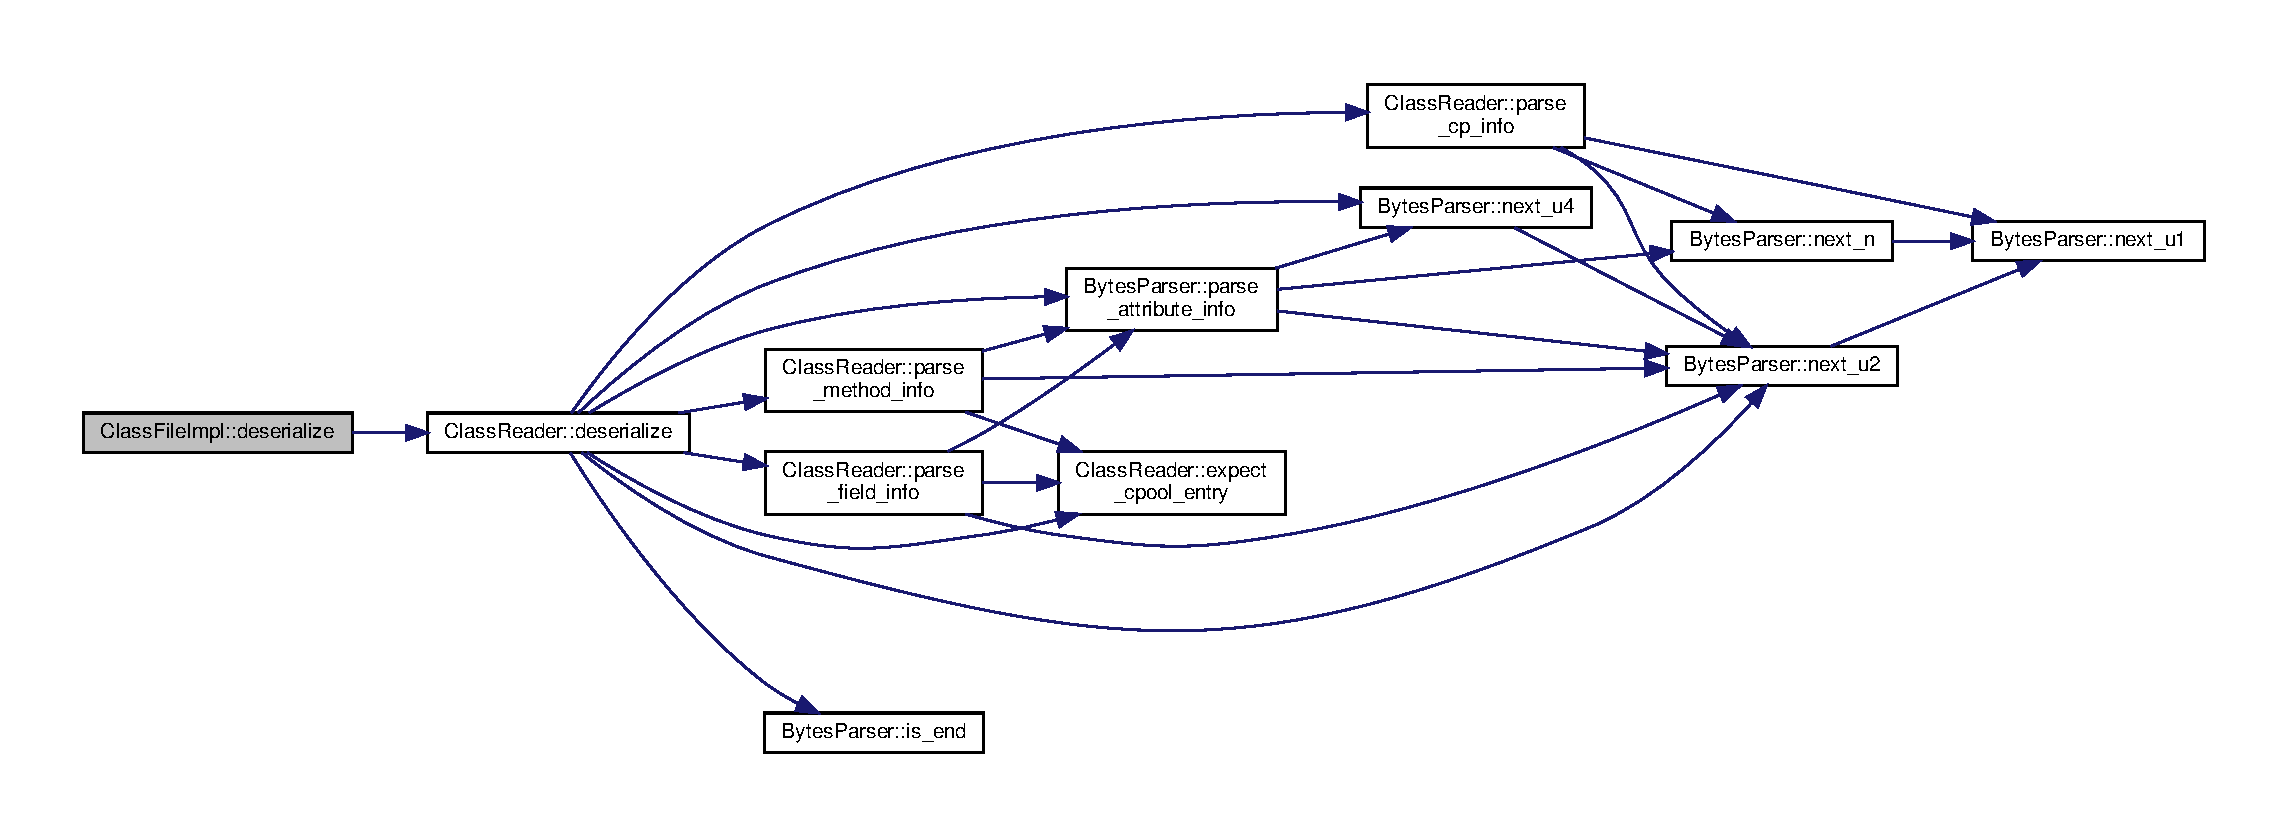
\includegraphics[width=350pt]{classClassFileImpl_abdfa46cef80b0ec30115f1c0c9bb1db6_cgraph}
\end{center}
\end{figure}
\mbox{\Hypertarget{classClassFileImpl_ad2154cb52119b87cd74b722b69730dee}\label{classClassFileImpl_ad2154cb52119b87cd74b722b69730dee}} 
\index{Class\+File\+Impl@{Class\+File\+Impl}!interface\+\_\+names@{interface\+\_\+names}}
\index{interface\+\_\+names@{interface\+\_\+names}!Class\+File\+Impl@{Class\+File\+Impl}}
\subsubsection{\texorpdfstring{interface\+\_\+names()}{interface\_names()}}
{\footnotesize\ttfamily std\+::vector$<$ std\+::string $>$ Class\+File\+Impl\+::interface\+\_\+names (\begin{DoxyParamCaption}{ }\end{DoxyParamCaption}) const}

Returns a vector containing the names of all the interfaces directly implemented by {\itshape this}. Note that this does not include transitive dependencies. Here is the call graph for this function\+:
\nopagebreak
\begin{figure}[H]
\begin{center}
\leavevmode
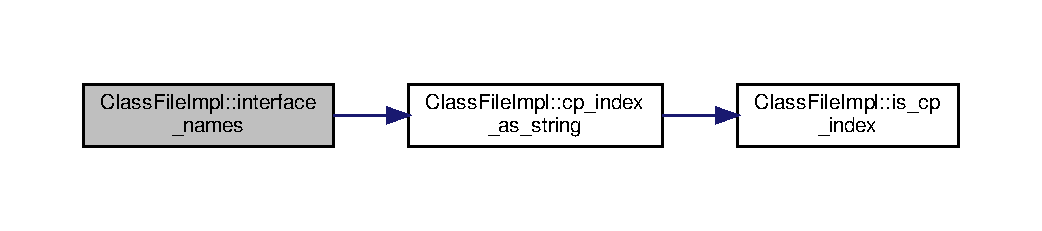
\includegraphics[width=350pt]{classClassFileImpl_ad2154cb52119b87cd74b722b69730dee_cgraph}
\end{center}
\end{figure}
\mbox{\Hypertarget{classClassFileImpl_a3772a57b8eaadf252a9a9f36c063ab93}\label{classClassFileImpl_a3772a57b8eaadf252a9a9f36c063ab93}} 
\index{Class\+File\+Impl@{Class\+File\+Impl}!is\+\_\+class@{is\+\_\+class}}
\index{is\+\_\+class@{is\+\_\+class}!Class\+File\+Impl@{Class\+File\+Impl}}
\subsubsection{\texorpdfstring{is\+\_\+class()}{is\_class()}}
{\footnotesize\ttfamily bool Class\+File\+Impl\+::is\+\_\+class (\begin{DoxyParamCaption}{ }\end{DoxyParamCaption}) const}

Returns whether this .class file represents an actual class, as opposed to an interface. Here is the call graph for this function\+:
\nopagebreak
\begin{figure}[H]
\begin{center}
\leavevmode
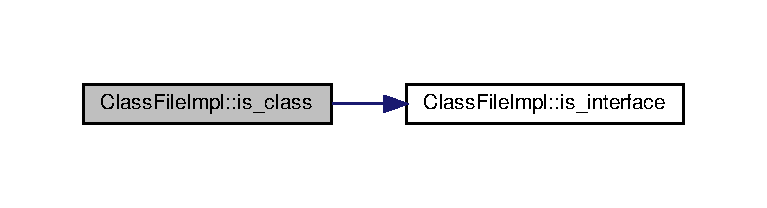
\includegraphics[width=350pt]{classClassFileImpl_a3772a57b8eaadf252a9a9f36c063ab93_cgraph}
\end{center}
\end{figure}
\mbox{\Hypertarget{classClassFileImpl_a1f15226f5107cb036e81d480531cda08}\label{classClassFileImpl_a1f15226f5107cb036e81d480531cda08}} 
\index{Class\+File\+Impl@{Class\+File\+Impl}!is\+\_\+cp\+\_\+index@{is\+\_\+cp\+\_\+index}}
\index{is\+\_\+cp\+\_\+index@{is\+\_\+cp\+\_\+index}!Class\+File\+Impl@{Class\+File\+Impl}}
\subsubsection{\texorpdfstring{is\+\_\+cp\+\_\+index()}{is\_cp\_index()}}
{\footnotesize\ttfamily bool Class\+File\+Impl\+::is\+\_\+cp\+\_\+index (\begin{DoxyParamCaption}\item[{int}]{index }\end{DoxyParamCaption}) const}

Returns whether {\ttfamily index} is actually an index into the constant pool array. \mbox{\Hypertarget{classClassFileImpl_ade64e9cb17003aa71ef596785ab8c575}\label{classClassFileImpl_ade64e9cb17003aa71ef596785ab8c575}} 
\index{Class\+File\+Impl@{Class\+File\+Impl}!is\+\_\+interface@{is\+\_\+interface}}
\index{is\+\_\+interface@{is\+\_\+interface}!Class\+File\+Impl@{Class\+File\+Impl}}
\subsubsection{\texorpdfstring{is\+\_\+interface()}{is\_interface()}}
{\footnotesize\ttfamily bool Class\+File\+Impl\+::is\+\_\+interface (\begin{DoxyParamCaption}{ }\end{DoxyParamCaption}) const}



Returns whether this is actually an interface, and not a class. 

\mbox{\Hypertarget{classClassFileImpl_ad8f4fcb051aa9d8c04d67373abe12c43}\label{classClassFileImpl_ad8f4fcb051aa9d8c04d67373abe12c43}} 
\index{Class\+File\+Impl@{Class\+File\+Impl}!is\+\_\+method\+\_\+index@{is\+\_\+method\+\_\+index}}
\index{is\+\_\+method\+\_\+index@{is\+\_\+method\+\_\+index}!Class\+File\+Impl@{Class\+File\+Impl}}
\subsubsection{\texorpdfstring{is\+\_\+method\+\_\+index()}{is\_method\_index()}}
{\footnotesize\ttfamily bool Class\+File\+Impl\+::is\+\_\+method\+\_\+index (\begin{DoxyParamCaption}\item[{int}]{index }\end{DoxyParamCaption}) const}



Returns whether {\ttfamily index} is actually an index into the methods array. 

\mbox{\Hypertarget{classClassFileImpl_a4e2a4657d4b102369ba7305251d41d00}\label{classClassFileImpl_a4e2a4657d4b102369ba7305251d41d00}} 
\index{Class\+File\+Impl@{Class\+File\+Impl}!serialize@{serialize}}
\index{serialize@{serialize}!Class\+File\+Impl@{Class\+File\+Impl}}
\subsubsection{\texorpdfstring{serialize()}{serialize()}}
{\footnotesize\ttfamily std\+::vector$<$ uint8\+\_\+t $>$ Class\+File\+Impl\+::serialize (\begin{DoxyParamCaption}{ }\end{DoxyParamCaption}) const}



Serialize the class file into binary data. 

Here is the call graph for this function\+:
\nopagebreak
\begin{figure}[H]
\begin{center}
\leavevmode
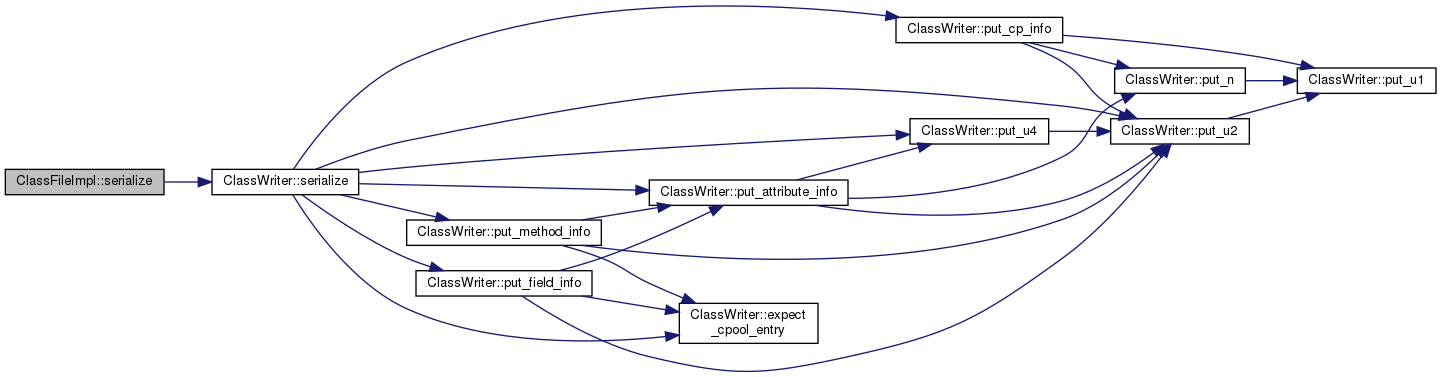
\includegraphics[width=350pt]{classClassFileImpl_a4e2a4657d4b102369ba7305251d41d00_cgraph}
\end{center}
\end{figure}
\mbox{\Hypertarget{classClassFileImpl_afd7229efcf341804086bcf6c00bb4820}\label{classClassFileImpl_afd7229efcf341804086bcf6c00bb4820}} 
\index{Class\+File\+Impl@{Class\+File\+Impl}!super\+\_\+class\+\_\+name@{super\+\_\+class\+\_\+name}}
\index{super\+\_\+class\+\_\+name@{super\+\_\+class\+\_\+name}!Class\+File\+Impl@{Class\+File\+Impl}}
\subsubsection{\texorpdfstring{super\+\_\+class\+\_\+name()}{super\_class\_name()}}
{\footnotesize\ttfamily std\+::string Class\+File\+Impl\+::super\+\_\+class\+\_\+name (\begin{DoxyParamCaption}{ }\end{DoxyParamCaption}) const}



Returns the name of the super class. 

Here is the call graph for this function\+:
\nopagebreak
\begin{figure}[H]
\begin{center}
\leavevmode
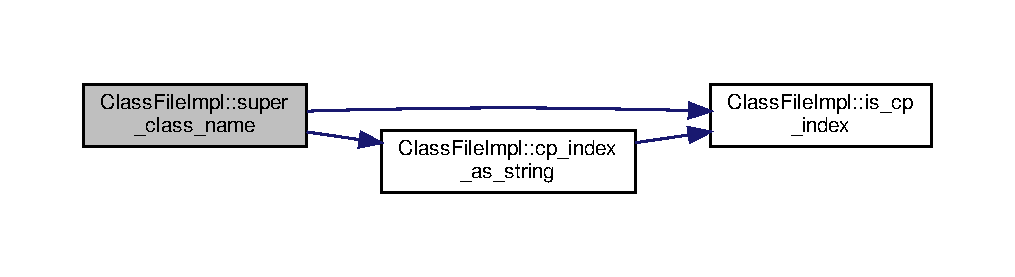
\includegraphics[width=350pt]{classClassFileImpl_afd7229efcf341804086bcf6c00bb4820_cgraph}
\end{center}
\end{figure}


\subsection{Member Data Documentation}
\mbox{\Hypertarget{classClassFileImpl_ae7bcc5b644d2164290c53a8727d36fb0}\label{classClassFileImpl_ae7bcc5b644d2164290c53a8727d36fb0}} 
\index{Class\+File\+Impl@{Class\+File\+Impl}!access\+\_\+flags@{access\+\_\+flags}}
\index{access\+\_\+flags@{access\+\_\+flags}!Class\+File\+Impl@{Class\+File\+Impl}}
\subsubsection{\texorpdfstring{access\+\_\+flags}{access\_flags}}
{\footnotesize\ttfamily \hyperlink{types_8h_ae676e9207f57fb921dca7366b2f59c53}{u2} Class\+File\+Impl\+::access\+\_\+flags}

\mbox{\Hypertarget{classClassFileImpl_ac1085cebfdbb8a2469d9de9782d0576d}\label{classClassFileImpl_ac1085cebfdbb8a2469d9de9782d0576d}} 
\index{Class\+File\+Impl@{Class\+File\+Impl}!attribute\+\_\+count@{attribute\+\_\+count}}
\index{attribute\+\_\+count@{attribute\+\_\+count}!Class\+File\+Impl@{Class\+File\+Impl}}
\subsubsection{\texorpdfstring{attribute\+\_\+count}{attribute\_count}}
{\footnotesize\ttfamily \hyperlink{types_8h_ae676e9207f57fb921dca7366b2f59c53}{u2} Class\+File\+Impl\+::attribute\+\_\+count}

\mbox{\Hypertarget{classClassFileImpl_a25689268cd6201a1b970a6dd41ac6fce}\label{classClassFileImpl_a25689268cd6201a1b970a6dd41ac6fce}} 
\index{Class\+File\+Impl@{Class\+File\+Impl}!attributes@{attributes}}
\index{attributes@{attributes}!Class\+File\+Impl@{Class\+File\+Impl}}
\subsubsection{\texorpdfstring{attributes}{attributes}}
{\footnotesize\ttfamily std\+::vector$<$\hyperlink{structattribute__info}{attribute\+\_\+info}$>$ Class\+File\+Impl\+::attributes}

\mbox{\Hypertarget{classClassFileImpl_ac3a364b19cfd1a647309dcf385e8d064}\label{classClassFileImpl_ac3a364b19cfd1a647309dcf385e8d064}} 
\index{Class\+File\+Impl@{Class\+File\+Impl}!constant\+\_\+pool@{constant\+\_\+pool}}
\index{constant\+\_\+pool@{constant\+\_\+pool}!Class\+File\+Impl@{Class\+File\+Impl}}
\subsubsection{\texorpdfstring{constant\+\_\+pool}{constant\_pool}}
{\footnotesize\ttfamily std\+::vector$<$\hyperlink{structcp__info}{cp\+\_\+info}$>$ Class\+File\+Impl\+::constant\+\_\+pool}

\mbox{\Hypertarget{classClassFileImpl_ad1cf3a358e54bf290b8602808f2d3a0b}\label{classClassFileImpl_ad1cf3a358e54bf290b8602808f2d3a0b}} 
\index{Class\+File\+Impl@{Class\+File\+Impl}!constant\+\_\+pool\+\_\+count@{constant\+\_\+pool\+\_\+count}}
\index{constant\+\_\+pool\+\_\+count@{constant\+\_\+pool\+\_\+count}!Class\+File\+Impl@{Class\+File\+Impl}}
\subsubsection{\texorpdfstring{constant\+\_\+pool\+\_\+count}{constant\_pool\_count}}
{\footnotesize\ttfamily \hyperlink{types_8h_ae676e9207f57fb921dca7366b2f59c53}{u2} Class\+File\+Impl\+::constant\+\_\+pool\+\_\+count}

\mbox{\Hypertarget{classClassFileImpl_a0144ff86144e3548e32779faf4e0dab9}\label{classClassFileImpl_a0144ff86144e3548e32779faf4e0dab9}} 
\index{Class\+File\+Impl@{Class\+File\+Impl}!field\+\_\+count@{field\+\_\+count}}
\index{field\+\_\+count@{field\+\_\+count}!Class\+File\+Impl@{Class\+File\+Impl}}
\subsubsection{\texorpdfstring{field\+\_\+count}{field\_count}}
{\footnotesize\ttfamily \hyperlink{types_8h_ae676e9207f57fb921dca7366b2f59c53}{u2} Class\+File\+Impl\+::field\+\_\+count}

\mbox{\Hypertarget{classClassFileImpl_af0ba1073f7566cdb21c47d33198ecab0}\label{classClassFileImpl_af0ba1073f7566cdb21c47d33198ecab0}} 
\index{Class\+File\+Impl@{Class\+File\+Impl}!fields@{fields}}
\index{fields@{fields}!Class\+File\+Impl@{Class\+File\+Impl}}
\subsubsection{\texorpdfstring{fields}{fields}}
{\footnotesize\ttfamily std\+::vector$<$\hyperlink{structfield__info}{field\+\_\+info}$>$ Class\+File\+Impl\+::fields}

\mbox{\Hypertarget{classClassFileImpl_ae8948beaa9ebac1d5df2c73ec62602c8}\label{classClassFileImpl_ae8948beaa9ebac1d5df2c73ec62602c8}} 
\index{Class\+File\+Impl@{Class\+File\+Impl}!interface\+\_\+count@{interface\+\_\+count}}
\index{interface\+\_\+count@{interface\+\_\+count}!Class\+File\+Impl@{Class\+File\+Impl}}
\subsubsection{\texorpdfstring{interface\+\_\+count}{interface\_count}}
{\footnotesize\ttfamily \hyperlink{types_8h_ae676e9207f57fb921dca7366b2f59c53}{u2} Class\+File\+Impl\+::interface\+\_\+count}

\mbox{\Hypertarget{classClassFileImpl_a449222435f48682e0f680432cf03f49b}\label{classClassFileImpl_a449222435f48682e0f680432cf03f49b}} 
\index{Class\+File\+Impl@{Class\+File\+Impl}!interfaces@{interfaces}}
\index{interfaces@{interfaces}!Class\+File\+Impl@{Class\+File\+Impl}}
\subsubsection{\texorpdfstring{interfaces}{interfaces}}
{\footnotesize\ttfamily std\+::vector$<$\hyperlink{structinterface__info}{interface\+\_\+info}$>$ Class\+File\+Impl\+::interfaces}

\mbox{\Hypertarget{classClassFileImpl_a31b4b986030442ae22f0630532032ded}\label{classClassFileImpl_a31b4b986030442ae22f0630532032ded}} 
\index{Class\+File\+Impl@{Class\+File\+Impl}!magic@{magic}}
\index{magic@{magic}!Class\+File\+Impl@{Class\+File\+Impl}}
\subsubsection{\texorpdfstring{magic}{magic}}
{\footnotesize\ttfamily \hyperlink{types_8h_af3b2d4b29fd9faedc984db3e062b3d5d}{u4} Class\+File\+Impl\+::magic}

\mbox{\Hypertarget{classClassFileImpl_ac48ee85570e9e8b06f7a568a4246c2da}\label{classClassFileImpl_ac48ee85570e9e8b06f7a568a4246c2da}} 
\index{Class\+File\+Impl@{Class\+File\+Impl}!major\+\_\+version@{major\+\_\+version}}
\index{major\+\_\+version@{major\+\_\+version}!Class\+File\+Impl@{Class\+File\+Impl}}
\subsubsection{\texorpdfstring{major\+\_\+version}{major\_version}}
{\footnotesize\ttfamily \hyperlink{types_8h_ae676e9207f57fb921dca7366b2f59c53}{u2} Class\+File\+Impl\+::major\+\_\+version}

\mbox{\Hypertarget{classClassFileImpl_a9643bb90606a32fa3f4a35f2ff468e5b}\label{classClassFileImpl_a9643bb90606a32fa3f4a35f2ff468e5b}} 
\index{Class\+File\+Impl@{Class\+File\+Impl}!method\+\_\+count@{method\+\_\+count}}
\index{method\+\_\+count@{method\+\_\+count}!Class\+File\+Impl@{Class\+File\+Impl}}
\subsubsection{\texorpdfstring{method\+\_\+count}{method\_count}}
{\footnotesize\ttfamily \hyperlink{types_8h_ae676e9207f57fb921dca7366b2f59c53}{u2} Class\+File\+Impl\+::method\+\_\+count}

\mbox{\Hypertarget{classClassFileImpl_a9142d753fc1a3b06ce26606506b2e9c1}\label{classClassFileImpl_a9142d753fc1a3b06ce26606506b2e9c1}} 
\index{Class\+File\+Impl@{Class\+File\+Impl}!methods@{methods}}
\index{methods@{methods}!Class\+File\+Impl@{Class\+File\+Impl}}
\subsubsection{\texorpdfstring{methods}{methods}}
{\footnotesize\ttfamily std\+::vector$<$\hyperlink{structmethod__info}{method\+\_\+info}$>$ Class\+File\+Impl\+::methods}

\mbox{\Hypertarget{classClassFileImpl_abec30809bc428ce5e31eebcd60a166e1}\label{classClassFileImpl_abec30809bc428ce5e31eebcd60a166e1}} 
\index{Class\+File\+Impl@{Class\+File\+Impl}!minor\+\_\+version@{minor\+\_\+version}}
\index{minor\+\_\+version@{minor\+\_\+version}!Class\+File\+Impl@{Class\+File\+Impl}}
\subsubsection{\texorpdfstring{minor\+\_\+version}{minor\_version}}
{\footnotesize\ttfamily \hyperlink{types_8h_ae676e9207f57fb921dca7366b2f59c53}{u2} Class\+File\+Impl\+::minor\+\_\+version}

\mbox{\Hypertarget{classClassFileImpl_aa85098174076217a362065cbf00d804b}\label{classClassFileImpl_aa85098174076217a362065cbf00d804b}} 
\index{Class\+File\+Impl@{Class\+File\+Impl}!super\+\_\+class@{super\+\_\+class}}
\index{super\+\_\+class@{super\+\_\+class}!Class\+File\+Impl@{Class\+File\+Impl}}
\subsubsection{\texorpdfstring{super\+\_\+class}{super\_class}}
{\footnotesize\ttfamily \hyperlink{types_8h_ae676e9207f57fb921dca7366b2f59c53}{u2} Class\+File\+Impl\+::super\+\_\+class}

\mbox{\Hypertarget{classClassFileImpl_a63d984dbdc45e796e6599e2c0b982f36}\label{classClassFileImpl_a63d984dbdc45e796e6599e2c0b982f36}} 
\index{Class\+File\+Impl@{Class\+File\+Impl}!this\+\_\+class@{this\+\_\+class}}
\index{this\+\_\+class@{this\+\_\+class}!Class\+File\+Impl@{Class\+File\+Impl}}
\subsubsection{\texorpdfstring{this\+\_\+class}{this\_class}}
{\footnotesize\ttfamily \hyperlink{types_8h_ae676e9207f57fb921dca7366b2f59c53}{u2} Class\+File\+Impl\+::this\+\_\+class}



The documentation for this class was generated from the following files\+:\begin{DoxyCompactItemize}
\item 
src/\hyperlink{classfile_8h}{classfile.\+h}\item 
src/\hyperlink{classfile_8cpp}{classfile.\+cpp}\end{DoxyCompactItemize}

\hypertarget{classClassReader}{}\section{Class\+Reader Class Reference}
\label{classClassReader}\index{Class\+Reader@{Class\+Reader}}


{\ttfamily \#include $<$classreader.\+h$>$}



Collaboration diagram for Class\+Reader\+:\nopagebreak
\begin{figure}[H]
\begin{center}
\leavevmode
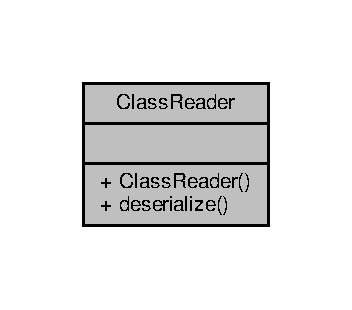
\includegraphics[height=550pt]{classClassReader__coll__graph}
\end{center}
\end{figure}
\subsection*{Public Member Functions}
\begin{DoxyCompactItemize}
\item 
\hyperlink{classClassReader_a3470778a3f6fe462416950a69c305ff0}{Class\+Reader} (std\+::vector$<$ uint8\+\_\+t $>$ data)
\begin{DoxyCompactList}\small\item\em Initialize the reader, with the binary {\ttfamily data} of the class file. \end{DoxyCompactList}\item 
\hyperlink{classClassFileImpl}{Class\+File\+Impl} \hyperlink{classClassReader_a001cc48324c31430559b43976d731e8a}{deserialize} ()
\end{DoxyCompactItemize}
\subsection*{Private Member Functions}
\begin{DoxyCompactItemize}
\item 
\hyperlink{structcp__info}{cp\+\_\+info} \hyperlink{classClassReader_ac4c0b613d45cf507b2e85c61c28541cb}{parse\+\_\+cp\+\_\+info} ()
\item 
\hyperlink{structfield__info}{field\+\_\+info} \hyperlink{classClassReader_a434b73f04e1502c936593ab63094d838}{parse\+\_\+field\+\_\+info} ()
\begin{DoxyCompactList}\small\item\em Parses a \hyperlink{structfield__info}{field\+\_\+info} struct from the data buffer. \end{DoxyCompactList}\item 
\hyperlink{structmethod__info}{method\+\_\+info} \hyperlink{classClassReader_a0eb68204b1979e2a2758c05f200a7be3}{parse\+\_\+method\+\_\+info} ()
\begin{DoxyCompactList}\small\item\em Parses a \hyperlink{structmethod__info}{method\+\_\+info} struct from the data buffer. \end{DoxyCompactList}\item 
void \hyperlink{classClassReader_a7f8a951758bdb961ebf36088301ac1b4}{expect\+\_\+cpool\+\_\+entry} (int idx, \hyperlink{structcp__info_acdef8472ed83e12e3a87bca8d6001f69}{cp\+\_\+info\+::\+Tag} tag) const
\end{DoxyCompactItemize}
\subsection*{Private Attributes}
\begin{DoxyCompactItemize}
\item 
\hyperlink{classBytesParser}{Bytes\+Parser} \hyperlink{classClassReader_a11f0ce7b430b8abd5cb74b4273ddaab0}{m\+\_\+bparser}
\begin{DoxyCompactList}\small\item\em The binary representation of the class being parser. \end{DoxyCompactList}\item 
\hyperlink{classClassFileImpl}{Class\+File\+Impl} \hyperlink{classClassReader_ad27b767f0ccf0826b0364977291894bc}{m\+\_\+cf}
\begin{DoxyCompactList}\small\item\em The class file that is being populated as the parsing progresses. \end{DoxyCompactList}\end{DoxyCompactItemize}


\subsection{Detailed Description}
This class handles the parsation (deserialization and serialization) of Java\textquotesingle{}s .class files. Normal usage should be\+:
\begin{DoxyEnumerate}
\item Reading the binary data (for example, from a file on disk)
\item Instantiating this \hyperlink{classClassReader}{Class\+Reader}.
\item Parsing the actual file. 
\end{DoxyEnumerate}

\subsection{Constructor \& Destructor Documentation}
\mbox{\Hypertarget{classClassReader_a3470778a3f6fe462416950a69c305ff0}\label{classClassReader_a3470778a3f6fe462416950a69c305ff0}} 
\index{Class\+Reader@{Class\+Reader}!Class\+Reader@{Class\+Reader}}
\index{Class\+Reader@{Class\+Reader}!Class\+Reader@{Class\+Reader}}
\subsubsection{\texorpdfstring{Class\+Reader()}{ClassReader()}}
{\footnotesize\ttfamily Class\+Reader\+::\+Class\+Reader (\begin{DoxyParamCaption}\item[{std\+::vector$<$ uint8\+\_\+t $>$}]{data }\end{DoxyParamCaption})}



Initialize the reader, with the binary {\ttfamily data} of the class file. 



\subsection{Member Function Documentation}
\mbox{\Hypertarget{classClassReader_a001cc48324c31430559b43976d731e8a}\label{classClassReader_a001cc48324c31430559b43976d731e8a}} 
\index{Class\+Reader@{Class\+Reader}!deserialize@{deserialize}}
\index{deserialize@{deserialize}!Class\+Reader@{Class\+Reader}}
\subsubsection{\texorpdfstring{deserialize()}{deserialize()}}
{\footnotesize\ttfamily \hyperlink{classClassFileImpl}{Class\+File\+Impl} Class\+Reader\+::deserialize (\begin{DoxyParamCaption}{ }\end{DoxyParamCaption})}

Parse an entire class file. This is the method that you most likely want to use. Here is the call graph for this function\+:\nopagebreak
\begin{figure}[H]
\begin{center}
\leavevmode
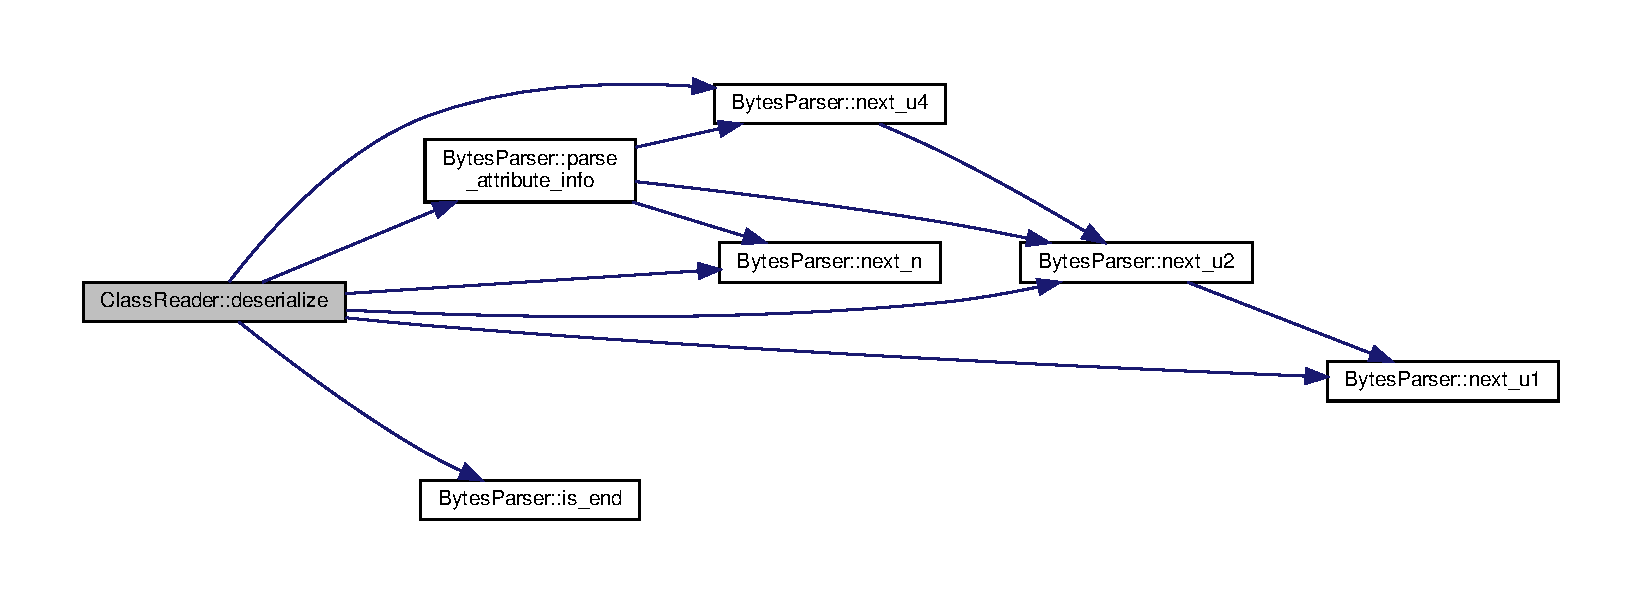
\includegraphics[width=350pt]{classClassReader_a001cc48324c31430559b43976d731e8a_cgraph}
\end{center}
\end{figure}
\mbox{\Hypertarget{classClassReader_a7f8a951758bdb961ebf36088301ac1b4}\label{classClassReader_a7f8a951758bdb961ebf36088301ac1b4}} 
\index{Class\+Reader@{Class\+Reader}!expect\+\_\+cpool\+\_\+entry@{expect\+\_\+cpool\+\_\+entry}}
\index{expect\+\_\+cpool\+\_\+entry@{expect\+\_\+cpool\+\_\+entry}!Class\+Reader@{Class\+Reader}}
\subsubsection{\texorpdfstring{expect\+\_\+cpool\+\_\+entry()}{expect\_cpool\_entry()}}
{\footnotesize\ttfamily void Class\+Reader\+::expect\+\_\+cpool\+\_\+entry (\begin{DoxyParamCaption}\item[{int}]{idx,  }\item[{\hyperlink{structcp__info_acdef8472ed83e12e3a87bca8d6001f69}{cp\+\_\+info\+::\+Tag}}]{tag }\end{DoxyParamCaption}) const\hspace{0.3cm}{\ttfamily [private]}}

Asserts that {\ttfamily idx} is an index into the constant pool, tagged with {\ttfamily tag}. \mbox{\Hypertarget{classClassReader_ac4c0b613d45cf507b2e85c61c28541cb}\label{classClassReader_ac4c0b613d45cf507b2e85c61c28541cb}} 
\index{Class\+Reader@{Class\+Reader}!parse\+\_\+cp\+\_\+info@{parse\+\_\+cp\+\_\+info}}
\index{parse\+\_\+cp\+\_\+info@{parse\+\_\+cp\+\_\+info}!Class\+Reader@{Class\+Reader}}
\subsubsection{\texorpdfstring{parse\+\_\+cp\+\_\+info()}{parse\_cp\_info()}}
{\footnotesize\ttfamily \hyperlink{structcp__info}{cp\+\_\+info} Class\+Reader\+::parse\+\_\+cp\+\_\+info (\begin{DoxyParamCaption}{ }\end{DoxyParamCaption})\hspace{0.3cm}{\ttfamily [private]}}

Parses a constant from the data buffer, and returns the data and how many slots it takes up in the constant table. Here is the call graph for this function\+:\nopagebreak
\begin{figure}[H]
\begin{center}
\leavevmode
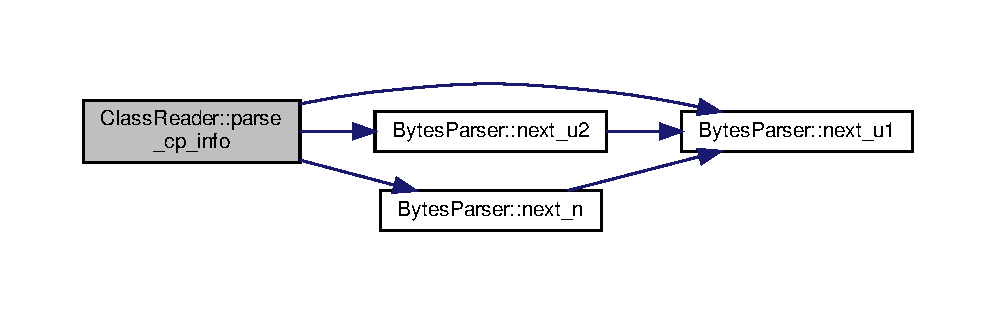
\includegraphics[width=350pt]{classClassReader_ac4c0b613d45cf507b2e85c61c28541cb_cgraph}
\end{center}
\end{figure}
\mbox{\Hypertarget{classClassReader_a434b73f04e1502c936593ab63094d838}\label{classClassReader_a434b73f04e1502c936593ab63094d838}} 
\index{Class\+Reader@{Class\+Reader}!parse\+\_\+field\+\_\+info@{parse\+\_\+field\+\_\+info}}
\index{parse\+\_\+field\+\_\+info@{parse\+\_\+field\+\_\+info}!Class\+Reader@{Class\+Reader}}
\subsubsection{\texorpdfstring{parse\+\_\+field\+\_\+info()}{parse\_field\_info()}}
{\footnotesize\ttfamily \hyperlink{structfield__info}{field\+\_\+info} Class\+Reader\+::parse\+\_\+field\+\_\+info (\begin{DoxyParamCaption}{ }\end{DoxyParamCaption})\hspace{0.3cm}{\ttfamily [private]}}



Parses a \hyperlink{structfield__info}{field\+\_\+info} struct from the data buffer. 

Here is the call graph for this function\+:\nopagebreak
\begin{figure}[H]
\begin{center}
\leavevmode
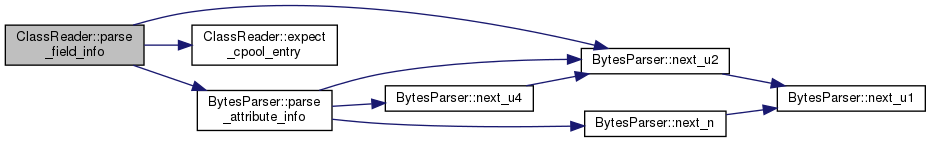
\includegraphics[width=350pt]{classClassReader_a434b73f04e1502c936593ab63094d838_cgraph}
\end{center}
\end{figure}
\mbox{\Hypertarget{classClassReader_a0eb68204b1979e2a2758c05f200a7be3}\label{classClassReader_a0eb68204b1979e2a2758c05f200a7be3}} 
\index{Class\+Reader@{Class\+Reader}!parse\+\_\+method\+\_\+info@{parse\+\_\+method\+\_\+info}}
\index{parse\+\_\+method\+\_\+info@{parse\+\_\+method\+\_\+info}!Class\+Reader@{Class\+Reader}}
\subsubsection{\texorpdfstring{parse\+\_\+method\+\_\+info()}{parse\_method\_info()}}
{\footnotesize\ttfamily \hyperlink{structmethod__info}{method\+\_\+info} Class\+Reader\+::parse\+\_\+method\+\_\+info (\begin{DoxyParamCaption}{ }\end{DoxyParamCaption})\hspace{0.3cm}{\ttfamily [private]}}



Parses a \hyperlink{structmethod__info}{method\+\_\+info} struct from the data buffer. 

Here is the call graph for this function\+:\nopagebreak
\begin{figure}[H]
\begin{center}
\leavevmode
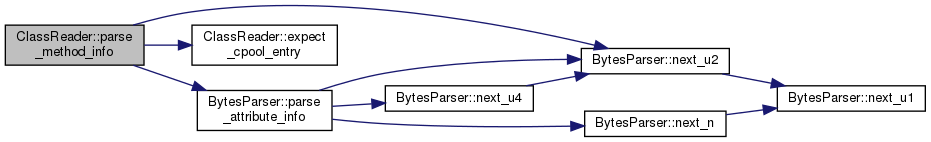
\includegraphics[width=350pt]{classClassReader_a0eb68204b1979e2a2758c05f200a7be3_cgraph}
\end{center}
\end{figure}


\subsection{Member Data Documentation}
\mbox{\Hypertarget{classClassReader_a11f0ce7b430b8abd5cb74b4273ddaab0}\label{classClassReader_a11f0ce7b430b8abd5cb74b4273ddaab0}} 
\index{Class\+Reader@{Class\+Reader}!m\+\_\+bparser@{m\+\_\+bparser}}
\index{m\+\_\+bparser@{m\+\_\+bparser}!Class\+Reader@{Class\+Reader}}
\subsubsection{\texorpdfstring{m\+\_\+bparser}{m\_bparser}}
{\footnotesize\ttfamily \hyperlink{classBytesParser}{Bytes\+Parser} Class\+Reader\+::m\+\_\+bparser\hspace{0.3cm}{\ttfamily [private]}}



The binary representation of the class being parser. 

\mbox{\Hypertarget{classClassReader_ad27b767f0ccf0826b0364977291894bc}\label{classClassReader_ad27b767f0ccf0826b0364977291894bc}} 
\index{Class\+Reader@{Class\+Reader}!m\+\_\+cf@{m\+\_\+cf}}
\index{m\+\_\+cf@{m\+\_\+cf}!Class\+Reader@{Class\+Reader}}
\subsubsection{\texorpdfstring{m\+\_\+cf}{m\_cf}}
{\footnotesize\ttfamily \hyperlink{classClassFileImpl}{Class\+File\+Impl} Class\+Reader\+::m\+\_\+cf\hspace{0.3cm}{\ttfamily [private]}}



The class file that is being populated as the parsing progresses. 



The documentation for this class was generated from the following files\+:\begin{DoxyCompactItemize}
\item 
src/\hyperlink{classreader_8h}{classreader.\+h}\item 
src/\hyperlink{classreader_8cpp}{classreader.\+cpp}\end{DoxyCompactItemize}

\hypertarget{classClassWriter}{}\section{Class\+Writer Class Reference}
\label{classClassWriter}\index{Class\+Writer@{Class\+Writer}}


{\ttfamily \#include $<$classwriter.\+h$>$}



Collaboration diagram for Class\+Writer\+:\nopagebreak
\begin{figure}[H]
\begin{center}
\leavevmode
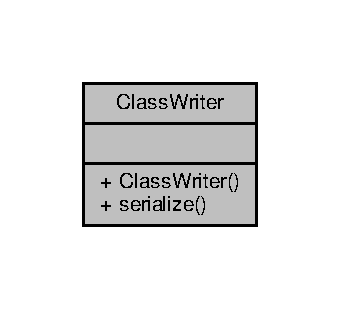
\includegraphics[height=550pt]{classClassWriter__coll__graph}
\end{center}
\end{figure}
\subsection*{Public Member Functions}
\begin{DoxyCompactItemize}
\item 
\hyperlink{classClassWriter_a4335e4ecbd5dfe24d08137201a87a298}{Class\+Writer} (const \hyperlink{classClassFileImpl}{Class\+File\+Impl} \&cf)
\begin{DoxyCompactList}\small\item\em Initialize the parser, with the binary {\ttfamily data} of the class file. \end{DoxyCompactList}\item 
std\+::vector$<$ uint8\+\_\+t $>$ \hyperlink{classClassWriter_a7be4d13b5665b1e85a8a350ec181951c}{serialize} ()
\end{DoxyCompactItemize}
\subsection*{Private Member Functions}
\begin{DoxyCompactItemize}
\item 
void \hyperlink{classClassWriter_a07332eb8e8e5ead72834e286cf8a6bd4}{put\+\_\+u1} (\hyperlink{types_8h_a162f47a77ee24f6f77cd8c82ccd40ab7}{u1} x)
\begin{DoxyCompactList}\small\item\em Puts an unsigned char into the data buffer, in network order. \end{DoxyCompactList}\item 
void \hyperlink{classClassWriter_a0304019dd68dd830fac5c67971ed2070}{put\+\_\+u2} (\hyperlink{types_8h_ae676e9207f57fb921dca7366b2f59c53}{u2} x)
\begin{DoxyCompactList}\small\item\em Puts an unsigned short into the data buffer, in network order. \end{DoxyCompactList}\item 
void \hyperlink{classClassWriter_aa6a42ab1ec0c2f85c30896506d6dbfce}{put\+\_\+u4} (\hyperlink{types_8h_af3b2d4b29fd9faedc984db3e062b3d5d}{u4} x)
\begin{DoxyCompactList}\small\item\em Puts an unsigned int into the data buffer, in network order. \end{DoxyCompactList}\item 
void \hyperlink{classClassWriter_aa527b917e9f3628ceaeccb95d30bfbb9}{put\+\_\+n} (const std\+::vector$<$ \hyperlink{types_8h_a162f47a77ee24f6f77cd8c82ccd40ab7}{u1} $>$ \&x)
\begin{DoxyCompactList}\small\item\em Puts the given vector into the data buffer. \end{DoxyCompactList}\item 
void \hyperlink{classClassWriter_a47741e12ae2af256ce3a58a41b2d04d6}{put\+\_\+cp\+\_\+info} (\hyperlink{structcp__info}{cp\+\_\+info} info)
\item 
void \hyperlink{classClassWriter_aeb256dbd55728dcc9081560691da779b}{put\+\_\+attribute\+\_\+info} (\hyperlink{structattribute__info}{attribute\+\_\+info} info)
\begin{DoxyCompactList}\small\item\em Puts an \hyperlink{structattribute__info}{attribute\+\_\+info} struct into the data buffer. \end{DoxyCompactList}\item 
void \hyperlink{classClassWriter_adfc5adcd821436ff9e399efac367c071}{put\+\_\+field\+\_\+info} (\hyperlink{structfield__info}{field\+\_\+info} info)
\begin{DoxyCompactList}\small\item\em Puts a \hyperlink{structfield__info}{field\+\_\+info} struct into the data buffer. \end{DoxyCompactList}\item 
void \hyperlink{classClassWriter_a3221090999bef5f0e05993de89600670}{put\+\_\+method\+\_\+info} (\hyperlink{structmethod__info}{method\+\_\+info} info)
\begin{DoxyCompactList}\small\item\em Puts a \hyperlink{structmethod__info}{method\+\_\+info} struct into the data buffer. \end{DoxyCompactList}\item 
void \hyperlink{classClassWriter_aa0d862bf0c0cdcdae72fd07444fa1e67}{expect\+\_\+cpool\+\_\+entry} (int idx, \hyperlink{structcp__info_acdef8472ed83e12e3a87bca8d6001f69}{cp\+\_\+info\+::\+Tag} tag) const
\end{DoxyCompactItemize}
\subsection*{Private Attributes}
\begin{DoxyCompactItemize}
\item 
const \hyperlink{classClassFileImpl}{Class\+File\+Impl} \& \hyperlink{classClassWriter_a4c495c4307d3634865d0a4d4024d4a37}{m\+\_\+cf}
\begin{DoxyCompactList}\small\item\em The class file that is used to generate the data. \end{DoxyCompactList}\item 
std\+::vector$<$ uint8\+\_\+t $>$ \hyperlink{classClassWriter_a8a5c126a562b0329307a15386ff389f8}{m\+\_\+data}
\begin{DoxyCompactList}\small\item\em The buffer that is being filled with the serialization data of {\ttfamily m\+\_\+cf}. \end{DoxyCompactList}\end{DoxyCompactItemize}


\subsection{Detailed Description}
This class handles the serialization of Java\textquotesingle{}s .class files. Normal usage should be\+: 

\subsection{Constructor \& Destructor Documentation}
\mbox{\Hypertarget{classClassWriter_a4335e4ecbd5dfe24d08137201a87a298}\label{classClassWriter_a4335e4ecbd5dfe24d08137201a87a298}} 
\index{Class\+Writer@{Class\+Writer}!Class\+Writer@{Class\+Writer}}
\index{Class\+Writer@{Class\+Writer}!Class\+Writer@{Class\+Writer}}
\subsubsection{\texorpdfstring{Class\+Writer()}{ClassWriter()}}
{\footnotesize\ttfamily Class\+Writer\+::\+Class\+Writer (\begin{DoxyParamCaption}\item[{const \hyperlink{classClassFileImpl}{Class\+File\+Impl} \&}]{cf }\end{DoxyParamCaption})}



Initialize the parser, with the binary {\ttfamily data} of the class file. 



\subsection{Member Function Documentation}
\mbox{\Hypertarget{classClassWriter_aa0d862bf0c0cdcdae72fd07444fa1e67}\label{classClassWriter_aa0d862bf0c0cdcdae72fd07444fa1e67}} 
\index{Class\+Writer@{Class\+Writer}!expect\+\_\+cpool\+\_\+entry@{expect\+\_\+cpool\+\_\+entry}}
\index{expect\+\_\+cpool\+\_\+entry@{expect\+\_\+cpool\+\_\+entry}!Class\+Writer@{Class\+Writer}}
\subsubsection{\texorpdfstring{expect\+\_\+cpool\+\_\+entry()}{expect\_cpool\_entry()}}
{\footnotesize\ttfamily void Class\+Writer\+::expect\+\_\+cpool\+\_\+entry (\begin{DoxyParamCaption}\item[{int}]{idx,  }\item[{\hyperlink{structcp__info_acdef8472ed83e12e3a87bca8d6001f69}{cp\+\_\+info\+::\+Tag}}]{tag }\end{DoxyParamCaption}) const\hspace{0.3cm}{\ttfamily [private]}}

Asserts that {\ttfamily idx} is an index into the constant pool, tagged with {\ttfamily tag}. \mbox{\Hypertarget{classClassWriter_aeb256dbd55728dcc9081560691da779b}\label{classClassWriter_aeb256dbd55728dcc9081560691da779b}} 
\index{Class\+Writer@{Class\+Writer}!put\+\_\+attribute\+\_\+info@{put\+\_\+attribute\+\_\+info}}
\index{put\+\_\+attribute\+\_\+info@{put\+\_\+attribute\+\_\+info}!Class\+Writer@{Class\+Writer}}
\subsubsection{\texorpdfstring{put\+\_\+attribute\+\_\+info()}{put\_attribute\_info()}}
{\footnotesize\ttfamily void Class\+Writer\+::put\+\_\+attribute\+\_\+info (\begin{DoxyParamCaption}\item[{\hyperlink{structattribute__info}{attribute\+\_\+info}}]{info }\end{DoxyParamCaption})\hspace{0.3cm}{\ttfamily [private]}}



Puts an \hyperlink{structattribute__info}{attribute\+\_\+info} struct into the data buffer. 

Here is the call graph for this function\+:\nopagebreak
\begin{figure}[H]
\begin{center}
\leavevmode
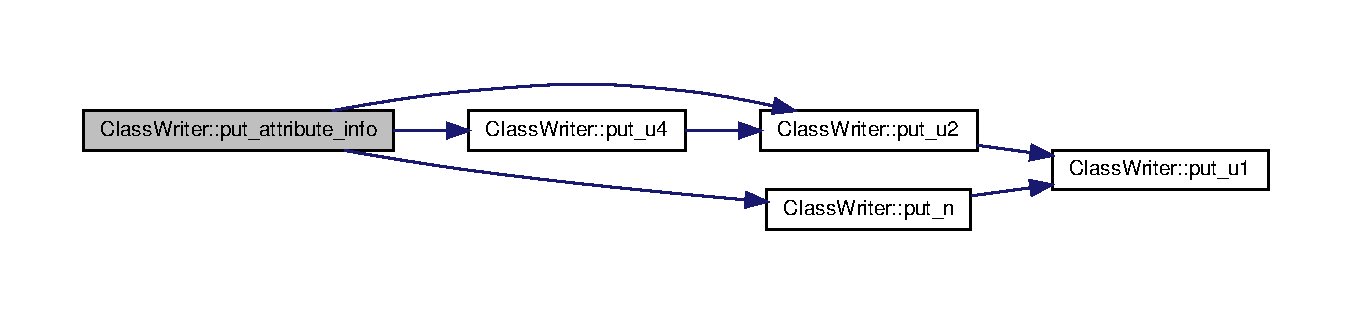
\includegraphics[width=350pt]{classClassWriter_aeb256dbd55728dcc9081560691da779b_cgraph}
\end{center}
\end{figure}
\mbox{\Hypertarget{classClassWriter_a47741e12ae2af256ce3a58a41b2d04d6}\label{classClassWriter_a47741e12ae2af256ce3a58a41b2d04d6}} 
\index{Class\+Writer@{Class\+Writer}!put\+\_\+cp\+\_\+info@{put\+\_\+cp\+\_\+info}}
\index{put\+\_\+cp\+\_\+info@{put\+\_\+cp\+\_\+info}!Class\+Writer@{Class\+Writer}}
\subsubsection{\texorpdfstring{put\+\_\+cp\+\_\+info()}{put\_cp\_info()}}
{\footnotesize\ttfamily void Class\+Writer\+::put\+\_\+cp\+\_\+info (\begin{DoxyParamCaption}\item[{\hyperlink{structcp__info}{cp\+\_\+info}}]{info }\end{DoxyParamCaption})\hspace{0.3cm}{\ttfamily [private]}}

Puts a constant from the data buffer, and returns the data and how many slots it takes up in the constant table. Here is the call graph for this function\+:\nopagebreak
\begin{figure}[H]
\begin{center}
\leavevmode
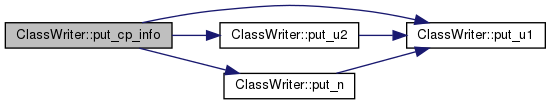
\includegraphics[width=350pt]{classClassWriter_a47741e12ae2af256ce3a58a41b2d04d6_cgraph}
\end{center}
\end{figure}
\mbox{\Hypertarget{classClassWriter_adfc5adcd821436ff9e399efac367c071}\label{classClassWriter_adfc5adcd821436ff9e399efac367c071}} 
\index{Class\+Writer@{Class\+Writer}!put\+\_\+field\+\_\+info@{put\+\_\+field\+\_\+info}}
\index{put\+\_\+field\+\_\+info@{put\+\_\+field\+\_\+info}!Class\+Writer@{Class\+Writer}}
\subsubsection{\texorpdfstring{put\+\_\+field\+\_\+info()}{put\_field\_info()}}
{\footnotesize\ttfamily void Class\+Writer\+::put\+\_\+field\+\_\+info (\begin{DoxyParamCaption}\item[{\hyperlink{structfield__info}{field\+\_\+info}}]{info }\end{DoxyParamCaption})\hspace{0.3cm}{\ttfamily [private]}}



Puts a \hyperlink{structfield__info}{field\+\_\+info} struct into the data buffer. 

Here is the call graph for this function\+:\nopagebreak
\begin{figure}[H]
\begin{center}
\leavevmode
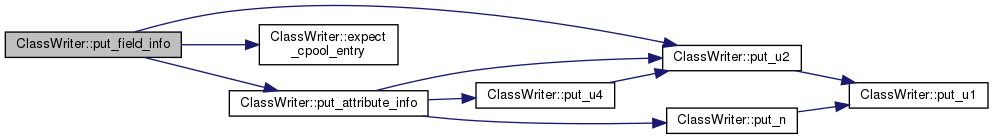
\includegraphics[width=350pt]{classClassWriter_adfc5adcd821436ff9e399efac367c071_cgraph}
\end{center}
\end{figure}
\mbox{\Hypertarget{classClassWriter_a3221090999bef5f0e05993de89600670}\label{classClassWriter_a3221090999bef5f0e05993de89600670}} 
\index{Class\+Writer@{Class\+Writer}!put\+\_\+method\+\_\+info@{put\+\_\+method\+\_\+info}}
\index{put\+\_\+method\+\_\+info@{put\+\_\+method\+\_\+info}!Class\+Writer@{Class\+Writer}}
\subsubsection{\texorpdfstring{put\+\_\+method\+\_\+info()}{put\_method\_info()}}
{\footnotesize\ttfamily void Class\+Writer\+::put\+\_\+method\+\_\+info (\begin{DoxyParamCaption}\item[{\hyperlink{structmethod__info}{method\+\_\+info}}]{info }\end{DoxyParamCaption})\hspace{0.3cm}{\ttfamily [private]}}



Puts a \hyperlink{structmethod__info}{method\+\_\+info} struct into the data buffer. 

Here is the call graph for this function\+:\nopagebreak
\begin{figure}[H]
\begin{center}
\leavevmode
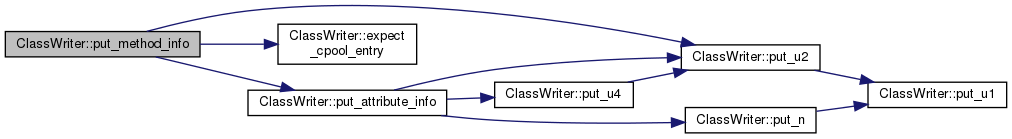
\includegraphics[width=350pt]{classClassWriter_a3221090999bef5f0e05993de89600670_cgraph}
\end{center}
\end{figure}
\mbox{\Hypertarget{classClassWriter_aa527b917e9f3628ceaeccb95d30bfbb9}\label{classClassWriter_aa527b917e9f3628ceaeccb95d30bfbb9}} 
\index{Class\+Writer@{Class\+Writer}!put\+\_\+n@{put\+\_\+n}}
\index{put\+\_\+n@{put\+\_\+n}!Class\+Writer@{Class\+Writer}}
\subsubsection{\texorpdfstring{put\+\_\+n()}{put\_n()}}
{\footnotesize\ttfamily void Class\+Writer\+::put\+\_\+n (\begin{DoxyParamCaption}\item[{const std\+::vector$<$ \hyperlink{types_8h_a162f47a77ee24f6f77cd8c82ccd40ab7}{u1} $>$ \&}]{x }\end{DoxyParamCaption})\hspace{0.3cm}{\ttfamily [private]}}



Puts the given vector into the data buffer. 

Here is the call graph for this function\+:\nopagebreak
\begin{figure}[H]
\begin{center}
\leavevmode
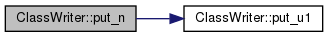
\includegraphics[width=318pt]{classClassWriter_aa527b917e9f3628ceaeccb95d30bfbb9_cgraph}
\end{center}
\end{figure}
\mbox{\Hypertarget{classClassWriter_a07332eb8e8e5ead72834e286cf8a6bd4}\label{classClassWriter_a07332eb8e8e5ead72834e286cf8a6bd4}} 
\index{Class\+Writer@{Class\+Writer}!put\+\_\+u1@{put\+\_\+u1}}
\index{put\+\_\+u1@{put\+\_\+u1}!Class\+Writer@{Class\+Writer}}
\subsubsection{\texorpdfstring{put\+\_\+u1()}{put\_u1()}}
{\footnotesize\ttfamily void Class\+Writer\+::put\+\_\+u1 (\begin{DoxyParamCaption}\item[{\hyperlink{types_8h_a162f47a77ee24f6f77cd8c82ccd40ab7}{u1}}]{x }\end{DoxyParamCaption})\hspace{0.3cm}{\ttfamily [private]}}



Puts an unsigned char into the data buffer, in network order. 

\mbox{\Hypertarget{classClassWriter_a0304019dd68dd830fac5c67971ed2070}\label{classClassWriter_a0304019dd68dd830fac5c67971ed2070}} 
\index{Class\+Writer@{Class\+Writer}!put\+\_\+u2@{put\+\_\+u2}}
\index{put\+\_\+u2@{put\+\_\+u2}!Class\+Writer@{Class\+Writer}}
\subsubsection{\texorpdfstring{put\+\_\+u2()}{put\_u2()}}
{\footnotesize\ttfamily void Class\+Writer\+::put\+\_\+u2 (\begin{DoxyParamCaption}\item[{\hyperlink{types_8h_ae676e9207f57fb921dca7366b2f59c53}{u2}}]{x }\end{DoxyParamCaption})\hspace{0.3cm}{\ttfamily [private]}}



Puts an unsigned short into the data buffer, in network order. 

Here is the call graph for this function\+:\nopagebreak
\begin{figure}[H]
\begin{center}
\leavevmode
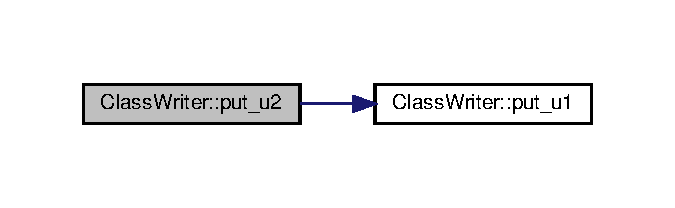
\includegraphics[width=324pt]{classClassWriter_a0304019dd68dd830fac5c67971ed2070_cgraph}
\end{center}
\end{figure}
\mbox{\Hypertarget{classClassWriter_aa6a42ab1ec0c2f85c30896506d6dbfce}\label{classClassWriter_aa6a42ab1ec0c2f85c30896506d6dbfce}} 
\index{Class\+Writer@{Class\+Writer}!put\+\_\+u4@{put\+\_\+u4}}
\index{put\+\_\+u4@{put\+\_\+u4}!Class\+Writer@{Class\+Writer}}
\subsubsection{\texorpdfstring{put\+\_\+u4()}{put\_u4()}}
{\footnotesize\ttfamily void Class\+Writer\+::put\+\_\+u4 (\begin{DoxyParamCaption}\item[{\hyperlink{types_8h_af3b2d4b29fd9faedc984db3e062b3d5d}{u4}}]{x }\end{DoxyParamCaption})\hspace{0.3cm}{\ttfamily [private]}}



Puts an unsigned int into the data buffer, in network order. 

Here is the call graph for this function\+:\nopagebreak
\begin{figure}[H]
\begin{center}
\leavevmode
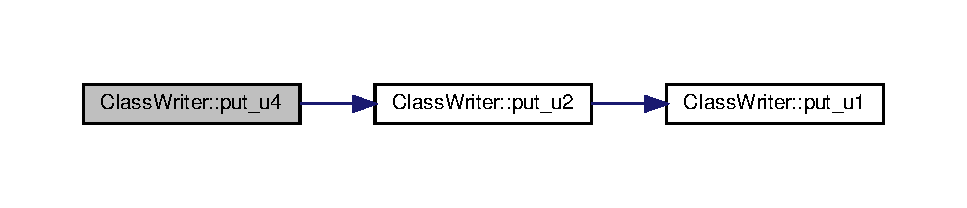
\includegraphics[width=350pt]{classClassWriter_aa6a42ab1ec0c2f85c30896506d6dbfce_cgraph}
\end{center}
\end{figure}
\mbox{\Hypertarget{classClassWriter_a7be4d13b5665b1e85a8a350ec181951c}\label{classClassWriter_a7be4d13b5665b1e85a8a350ec181951c}} 
\index{Class\+Writer@{Class\+Writer}!serialize@{serialize}}
\index{serialize@{serialize}!Class\+Writer@{Class\+Writer}}
\subsubsection{\texorpdfstring{serialize()}{serialize()}}
{\footnotesize\ttfamily std\+::vector$<$ uint8\+\_\+t $>$ Class\+Writer\+::serialize (\begin{DoxyParamCaption}{ }\end{DoxyParamCaption})}

Parse an entire class file. This is the method that you most likely want to use. Here is the call graph for this function\+:\nopagebreak
\begin{figure}[H]
\begin{center}
\leavevmode
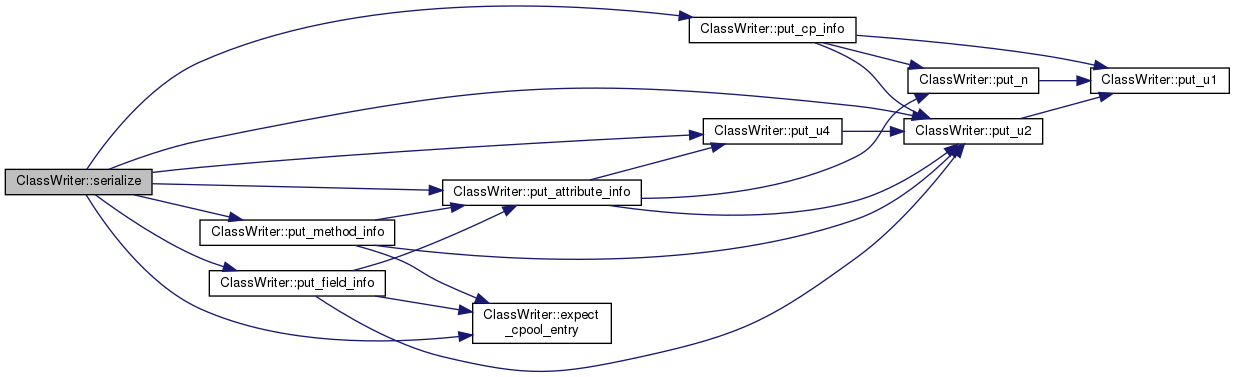
\includegraphics[width=350pt]{classClassWriter_a7be4d13b5665b1e85a8a350ec181951c_cgraph}
\end{center}
\end{figure}


\subsection{Member Data Documentation}
\mbox{\Hypertarget{classClassWriter_a4c495c4307d3634865d0a4d4024d4a37}\label{classClassWriter_a4c495c4307d3634865d0a4d4024d4a37}} 
\index{Class\+Writer@{Class\+Writer}!m\+\_\+cf@{m\+\_\+cf}}
\index{m\+\_\+cf@{m\+\_\+cf}!Class\+Writer@{Class\+Writer}}
\subsubsection{\texorpdfstring{m\+\_\+cf}{m\_cf}}
{\footnotesize\ttfamily const \hyperlink{classClassFileImpl}{Class\+File\+Impl}\& Class\+Writer\+::m\+\_\+cf\hspace{0.3cm}{\ttfamily [private]}}



The class file that is used to generate the data. 

\mbox{\Hypertarget{classClassWriter_a8a5c126a562b0329307a15386ff389f8}\label{classClassWriter_a8a5c126a562b0329307a15386ff389f8}} 
\index{Class\+Writer@{Class\+Writer}!m\+\_\+data@{m\+\_\+data}}
\index{m\+\_\+data@{m\+\_\+data}!Class\+Writer@{Class\+Writer}}
\subsubsection{\texorpdfstring{m\+\_\+data}{m\_data}}
{\footnotesize\ttfamily std\+::vector$<$uint8\+\_\+t$>$ Class\+Writer\+::m\+\_\+data\hspace{0.3cm}{\ttfamily [private]}}



The buffer that is being filled with the serialization data of {\ttfamily m\+\_\+cf}. 



The documentation for this class was generated from the following files\+:\begin{DoxyCompactItemize}
\item 
src/\hyperlink{classwriter_8h}{classwriter.\+h}\item 
src/\hyperlink{classwriter_8cpp}{classwriter.\+cpp}\end{DoxyCompactItemize}

\hypertarget{structCode__attribute}{}\section{Code\+\_\+attribute Struct Reference}
\label{structCode__attribute}\index{Code\+\_\+attribute@{Code\+\_\+attribute}}


Collaboration diagram for Code\+\_\+attribute\+:
\nopagebreak
\begin{figure}[H]
\begin{center}
\leavevmode
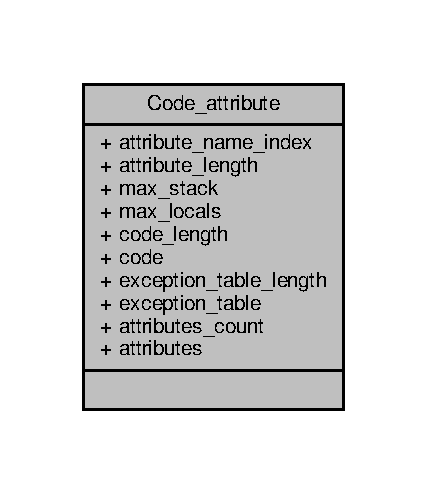
\includegraphics[width=205pt]{structCode__attribute__coll__graph}
\end{center}
\end{figure}
\subsection*{Classes}
\begin{DoxyCompactItemize}
\item 
struct \hyperlink{structCode__attribute_1_1exception}{exception}
\end{DoxyCompactItemize}


The documentation for this struct was generated from the following file\+:\begin{DoxyCompactItemize}
\item 
src/types.\+h\end{DoxyCompactItemize}

\hypertarget{structCONSTANT__Class__info}{}\section{C\+O\+N\+S\+T\+A\+N\+T\+\_\+\+Class\+\_\+info Struct Reference}
\label{structCONSTANT__Class__info}\index{C\+O\+N\+S\+T\+A\+N\+T\+\_\+\+Class\+\_\+info@{C\+O\+N\+S\+T\+A\+N\+T\+\_\+\+Class\+\_\+info}}


Collaboration diagram for C\+O\+N\+S\+T\+A\+N\+T\+\_\+\+Class\+\_\+info\+:
\nopagebreak
\begin{figure}[H]
\begin{center}
\leavevmode
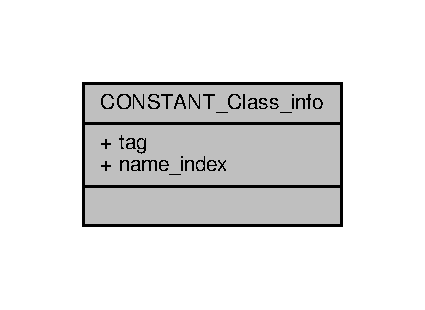
\includegraphics[width=204pt]{structCONSTANT__Class__info__coll__graph}
\end{center}
\end{figure}


The documentation for this struct was generated from the following file\+:\begin{DoxyCompactItemize}
\item 
src/types.\+h\end{DoxyCompactItemize}

\hypertarget{structCONSTANT__GenericMethodref__info}{}\section{C\+O\+N\+S\+T\+A\+N\+T\+\_\+\+Generic\+Methodref\+\_\+info Struct Reference}
\label{structCONSTANT__GenericMethodref__info}\index{C\+O\+N\+S\+T\+A\+N\+T\+\_\+\+Generic\+Methodref\+\_\+info@{C\+O\+N\+S\+T\+A\+N\+T\+\_\+\+Generic\+Methodref\+\_\+info}}


{\ttfamily \#include $<$types.\+h$>$}



Collaboration diagram for C\+O\+N\+S\+T\+A\+N\+T\+\_\+\+Generic\+Methodref\+\_\+info\+:\nopagebreak
\begin{figure}[H]
\begin{center}
\leavevmode
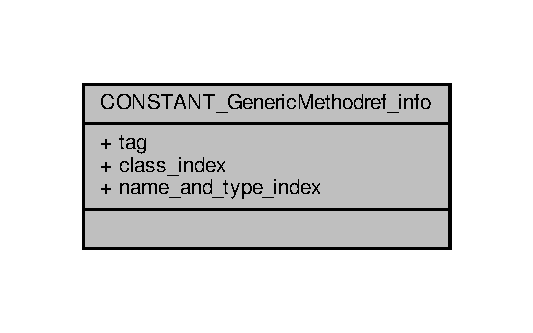
\includegraphics[width=256pt]{structCONSTANT__GenericMethodref__info__coll__graph}
\end{center}
\end{figure}


\subsection{Detailed Description}
Although Methodref and Interface\+Methodref are semantically different, they have the same layout and even the same field names. For the scope of this project, we can treat them as pretty much the same thing. 

The documentation for this struct was generated from the following file\+:\begin{DoxyCompactItemize}
\item 
src/types.\+h\end{DoxyCompactItemize}

\hypertarget{structCONSTANT__NameAndType__info}{}\section{C\+O\+N\+S\+T\+A\+N\+T\+\_\+\+Name\+And\+Type\+\_\+info Struct Reference}
\label{structCONSTANT__NameAndType__info}\index{C\+O\+N\+S\+T\+A\+N\+T\+\_\+\+Name\+And\+Type\+\_\+info@{C\+O\+N\+S\+T\+A\+N\+T\+\_\+\+Name\+And\+Type\+\_\+info}}


{\ttfamily \#include $<$types.\+h$>$}



Collaboration diagram for C\+O\+N\+S\+T\+A\+N\+T\+\_\+\+Name\+And\+Type\+\_\+info\+:\nopagebreak
\begin{figure}[H]
\begin{center}
\leavevmode
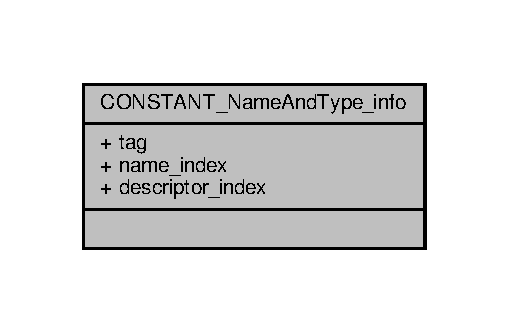
\includegraphics[width=244pt]{structCONSTANT__NameAndType__info__coll__graph}
\end{center}
\end{figure}
\subsection*{Public Attributes}
\begin{DoxyCompactItemize}
\item 
\hyperlink{structcp__info_acdef8472ed83e12e3a87bca8d6001f69}{cp\+\_\+info\+::\+Tag} \hyperlink{structCONSTANT__NameAndType__info_a5a4f7d881529f76682bf58fd56d34d29}{tag}
\item 
\hyperlink{types_8h_ae676e9207f57fb921dca7366b2f59c53}{u2} \hyperlink{structCONSTANT__NameAndType__info_adbaa813f9f3a32dc04a8bc65b5b2433d}{name\+\_\+index}
\item 
\hyperlink{types_8h_ae676e9207f57fb921dca7366b2f59c53}{u2} \hyperlink{structCONSTANT__NameAndType__info_a5066151677d138f5ee57e5e16efd4d5e}{descriptor\+\_\+index}
\end{DoxyCompactItemize}


\subsection{Member Data Documentation}
\mbox{\Hypertarget{structCONSTANT__NameAndType__info_a5066151677d138f5ee57e5e16efd4d5e}\label{structCONSTANT__NameAndType__info_a5066151677d138f5ee57e5e16efd4d5e}} 
\index{C\+O\+N\+S\+T\+A\+N\+T\+\_\+\+Name\+And\+Type\+\_\+info@{C\+O\+N\+S\+T\+A\+N\+T\+\_\+\+Name\+And\+Type\+\_\+info}!descriptor\+\_\+index@{descriptor\+\_\+index}}
\index{descriptor\+\_\+index@{descriptor\+\_\+index}!C\+O\+N\+S\+T\+A\+N\+T\+\_\+\+Name\+And\+Type\+\_\+info@{C\+O\+N\+S\+T\+A\+N\+T\+\_\+\+Name\+And\+Type\+\_\+info}}
\subsubsection{\texorpdfstring{descriptor\+\_\+index}{descriptor\_index}}
{\footnotesize\ttfamily \hyperlink{types_8h_ae676e9207f57fb921dca7366b2f59c53}{u2} C\+O\+N\+S\+T\+A\+N\+T\+\_\+\+Name\+And\+Type\+\_\+info\+::descriptor\+\_\+index}

\mbox{\Hypertarget{structCONSTANT__NameAndType__info_adbaa813f9f3a32dc04a8bc65b5b2433d}\label{structCONSTANT__NameAndType__info_adbaa813f9f3a32dc04a8bc65b5b2433d}} 
\index{C\+O\+N\+S\+T\+A\+N\+T\+\_\+\+Name\+And\+Type\+\_\+info@{C\+O\+N\+S\+T\+A\+N\+T\+\_\+\+Name\+And\+Type\+\_\+info}!name\+\_\+index@{name\+\_\+index}}
\index{name\+\_\+index@{name\+\_\+index}!C\+O\+N\+S\+T\+A\+N\+T\+\_\+\+Name\+And\+Type\+\_\+info@{C\+O\+N\+S\+T\+A\+N\+T\+\_\+\+Name\+And\+Type\+\_\+info}}
\subsubsection{\texorpdfstring{name\+\_\+index}{name\_index}}
{\footnotesize\ttfamily \hyperlink{types_8h_ae676e9207f57fb921dca7366b2f59c53}{u2} C\+O\+N\+S\+T\+A\+N\+T\+\_\+\+Name\+And\+Type\+\_\+info\+::name\+\_\+index}

\mbox{\Hypertarget{structCONSTANT__NameAndType__info_a5a4f7d881529f76682bf58fd56d34d29}\label{structCONSTANT__NameAndType__info_a5a4f7d881529f76682bf58fd56d34d29}} 
\index{C\+O\+N\+S\+T\+A\+N\+T\+\_\+\+Name\+And\+Type\+\_\+info@{C\+O\+N\+S\+T\+A\+N\+T\+\_\+\+Name\+And\+Type\+\_\+info}!tag@{tag}}
\index{tag@{tag}!C\+O\+N\+S\+T\+A\+N\+T\+\_\+\+Name\+And\+Type\+\_\+info@{C\+O\+N\+S\+T\+A\+N\+T\+\_\+\+Name\+And\+Type\+\_\+info}}
\subsubsection{\texorpdfstring{tag}{tag}}
{\footnotesize\ttfamily \hyperlink{structcp__info_acdef8472ed83e12e3a87bca8d6001f69}{cp\+\_\+info\+::\+Tag} C\+O\+N\+S\+T\+A\+N\+T\+\_\+\+Name\+And\+Type\+\_\+info\+::tag}



The documentation for this struct was generated from the following file\+:\begin{DoxyCompactItemize}
\item 
src/\hyperlink{types_8h}{types.\+h}\end{DoxyCompactItemize}

\hypertarget{structcp__info}{}\section{cp\+\_\+info Struct Reference}
\label{structcp__info}\index{cp\+\_\+info@{cp\+\_\+info}}


{\ttfamily \#include $<$types.\+h$>$}



Collaboration diagram for cp\+\_\+info\+:\nopagebreak
\begin{figure}[H]
\begin{center}
\leavevmode
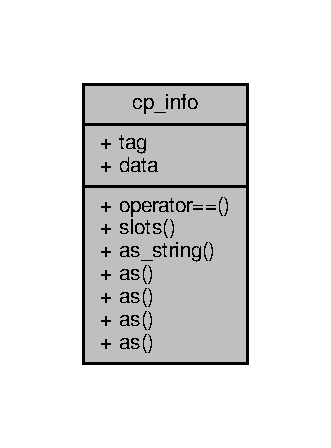
\includegraphics[width=159pt]{structcp__info__coll__graph}
\end{center}
\end{figure}
\subsection*{Public Types}
\begin{DoxyCompactItemize}
\item 
enum \hyperlink{structcp__info_acdef8472ed83e12e3a87bca8d6001f69}{Tag} \+: u1 \{ \newline
\hyperlink{structcp__info_acdef8472ed83e12e3a87bca8d6001f69adf4763ef84792f4fab0a07fcb179de22}{Tag\+::\+C\+O\+N\+S\+T\+A\+N\+T\+\_\+\+Class} = 7, 
\hyperlink{structcp__info_acdef8472ed83e12e3a87bca8d6001f69ac4a7343d330901c964bc6d7a100d0e07}{Tag\+::\+C\+O\+N\+S\+T\+A\+N\+T\+\_\+\+Fieldref} = 9, 
\hyperlink{structcp__info_acdef8472ed83e12e3a87bca8d6001f69a134e81d65f8cc7c04abcbc28ecb5ebf6}{Tag\+::\+C\+O\+N\+S\+T\+A\+N\+T\+\_\+\+Methodref} = 10, 
\hyperlink{structcp__info_acdef8472ed83e12e3a87bca8d6001f69a475c27d2bacb9d567842963d43c30ae2}{Tag\+::\+C\+O\+N\+S\+T\+A\+N\+T\+\_\+\+Interface\+Methodref} = 11, 
\newline
\hyperlink{structcp__info_acdef8472ed83e12e3a87bca8d6001f69ab084121ff44655538433e0092625b757}{Tag\+::\+C\+O\+N\+S\+T\+A\+N\+T\+\_\+\+String} = 8, 
\hyperlink{structcp__info_acdef8472ed83e12e3a87bca8d6001f69ae657037d317a6128b92247bd0b07c300}{Tag\+::\+C\+O\+N\+S\+T\+A\+N\+T\+\_\+\+Integer} = 3, 
\hyperlink{structcp__info_acdef8472ed83e12e3a87bca8d6001f69a706b340607da83ec3ae76605dd27b722}{Tag\+::\+C\+O\+N\+S\+T\+A\+N\+T\+\_\+\+Float} = 4, 
\hyperlink{structcp__info_acdef8472ed83e12e3a87bca8d6001f69a19c30801e986993747aabd3327b7a623}{Tag\+::\+C\+O\+N\+S\+T\+A\+N\+T\+\_\+\+Long} = 5, 
\newline
\hyperlink{structcp__info_acdef8472ed83e12e3a87bca8d6001f69a71cd8d4c23581349260ab388e6629e98}{Tag\+::\+C\+O\+N\+S\+T\+A\+N\+T\+\_\+\+Double} = 6, 
\hyperlink{structcp__info_acdef8472ed83e12e3a87bca8d6001f69a454459b9eeb1bf297d97d91b04275643}{Tag\+::\+C\+O\+N\+S\+T\+A\+N\+T\+\_\+\+Name\+And\+Type} = 12, 
\hyperlink{structcp__info_acdef8472ed83e12e3a87bca8d6001f69a9b59fd6f1baef2be4b10cb0cfdffb4be}{Tag\+::\+C\+O\+N\+S\+T\+A\+N\+T\+\_\+\+Utf8\+\_\+info} = 1, 
\hyperlink{structcp__info_acdef8472ed83e12e3a87bca8d6001f69a3c5a3d3a1f2c967a7eadba51cef03549}{Tag\+::\+C\+O\+N\+S\+T\+A\+N\+T\+\_\+\+Method\+Handle} = 15, 
\newline
\hyperlink{structcp__info_acdef8472ed83e12e3a87bca8d6001f69adbdbd6fda169a3ae47194edf8d99ba0d}{Tag\+::\+C\+O\+N\+S\+T\+A\+N\+T\+\_\+\+Method\+Type} = 16, 
\hyperlink{structcp__info_acdef8472ed83e12e3a87bca8d6001f69a4820a591c800d6e0ed560e18ac786969}{Tag\+::\+C\+O\+N\+S\+T\+A\+N\+T\+\_\+\+Invoke\+Dynamic} = 18
 \}
\end{DoxyCompactItemize}
\subsection*{Public Member Functions}
\begin{DoxyCompactItemize}
\item 
bool \hyperlink{structcp__info_a486b4be323e8194d6efcf388f3533fb1}{operator==} (const \hyperlink{structcp__info}{cp\+\_\+info} \&other) const
\item 
int \hyperlink{structcp__info_a1371b901a960486462d8cc6efc0c6ee8}{slots} () const
\item 
std\+::string \hyperlink{structcp__info_a8bdd7454a673dea621f24569c4c6aa01}{as\+\_\+string} () const
\begin{DoxyCompactList}\small\item\em Returns {\itshape this} as string. \end{DoxyCompactList}\item 
{\footnotesize template$<$typename T $>$ }\\T \hyperlink{structcp__info_a73e88cec575d05a03d73cbfcc91cd71b}{as} () const
\begin{DoxyCompactList}\small\item\em This template will be explicitly specialized for the possible types. \end{DoxyCompactList}\item 
{\footnotesize template$<$$>$ }\\\hyperlink{structCONSTANT__GenericMethodref__info}{C\+O\+N\+S\+T\+A\+N\+T\+\_\+\+Generic\+Methodref\+\_\+info} \hyperlink{structcp__info_a032c6014839b743ea813f1e69df0e478}{as} () const
\item 
{\footnotesize template$<$$>$ }\\\hyperlink{structCONSTANT__Class__info}{C\+O\+N\+S\+T\+A\+N\+T\+\_\+\+Class\+\_\+info} \hyperlink{structcp__info_aa1c10a3fe7a296f25f0f25eb30d96979}{as} () const
\item 
{\footnotesize template$<$$>$ }\\\hyperlink{structCONSTANT__NameAndType__info}{C\+O\+N\+S\+T\+A\+N\+T\+\_\+\+Name\+And\+Type\+\_\+info} \hyperlink{structcp__info_af14ec722b429cf5cb5b7fc52a7a955b8}{as} () const
\end{DoxyCompactItemize}
\subsection*{Public Attributes}
\begin{DoxyCompactItemize}
\item 
\hyperlink{structcp__info_acdef8472ed83e12e3a87bca8d6001f69}{Tag} \hyperlink{structcp__info_a9d61bf7aad6935bfe368e4ec509af6ec}{tag}
\item 
std\+::vector$<$ \hyperlink{types_8h_a162f47a77ee24f6f77cd8c82ccd40ab7}{u1} $>$ \hyperlink{structcp__info_aca6cdfc0ccd687b71c824415258bc870}{data}
\end{DoxyCompactItemize}


\subsection{Detailed Description}
Each item in the constant\+\_\+pool table must begin with a 1-\/byte tag indicating the kind of \hyperlink{structcp__info}{cp\+\_\+info} entry. The contents of the info array vary with the value of tag. The valid tags and their values are included in the tag enum. Each tag byte must be followed by two or more bytes giving information about the specific constant. The format of the additional information varies with the tag value. 

\subsection{Member Enumeration Documentation}
\mbox{\Hypertarget{structcp__info_acdef8472ed83e12e3a87bca8d6001f69}\label{structcp__info_acdef8472ed83e12e3a87bca8d6001f69}} 
\index{cp\+\_\+info@{cp\+\_\+info}!Tag@{Tag}}
\index{Tag@{Tag}!cp\+\_\+info@{cp\+\_\+info}}
\subsubsection{\texorpdfstring{Tag}{Tag}}
{\footnotesize\ttfamily enum \hyperlink{structcp__info_acdef8472ed83e12e3a87bca8d6001f69}{cp\+\_\+info\+::\+Tag} \+: \hyperlink{types_8h_a162f47a77ee24f6f77cd8c82ccd40ab7}{u1}\hspace{0.3cm}{\ttfamily [strong]}}

\begin{DoxyEnumFields}{Enumerator}
\raisebox{\heightof{T}}[0pt][0pt]{\index{C\+O\+N\+S\+T\+A\+N\+T\+\_\+\+Class@{C\+O\+N\+S\+T\+A\+N\+T\+\_\+\+Class}!cp\+\_\+info@{cp\+\_\+info}}\index{cp\+\_\+info@{cp\+\_\+info}!C\+O\+N\+S\+T\+A\+N\+T\+\_\+\+Class@{C\+O\+N\+S\+T\+A\+N\+T\+\_\+\+Class}}}\mbox{\Hypertarget{structcp__info_acdef8472ed83e12e3a87bca8d6001f69adf4763ef84792f4fab0a07fcb179de22}\label{structcp__info_acdef8472ed83e12e3a87bca8d6001f69adf4763ef84792f4fab0a07fcb179de22}} 
C\+O\+N\+S\+T\+A\+N\+T\+\_\+\+Class&\\
\hline

\raisebox{\heightof{T}}[0pt][0pt]{\index{C\+O\+N\+S\+T\+A\+N\+T\+\_\+\+Fieldref@{C\+O\+N\+S\+T\+A\+N\+T\+\_\+\+Fieldref}!cp\+\_\+info@{cp\+\_\+info}}\index{cp\+\_\+info@{cp\+\_\+info}!C\+O\+N\+S\+T\+A\+N\+T\+\_\+\+Fieldref@{C\+O\+N\+S\+T\+A\+N\+T\+\_\+\+Fieldref}}}\mbox{\Hypertarget{structcp__info_acdef8472ed83e12e3a87bca8d6001f69ac4a7343d330901c964bc6d7a100d0e07}\label{structcp__info_acdef8472ed83e12e3a87bca8d6001f69ac4a7343d330901c964bc6d7a100d0e07}} 
C\+O\+N\+S\+T\+A\+N\+T\+\_\+\+Fieldref&\\
\hline

\raisebox{\heightof{T}}[0pt][0pt]{\index{C\+O\+N\+S\+T\+A\+N\+T\+\_\+\+Methodref@{C\+O\+N\+S\+T\+A\+N\+T\+\_\+\+Methodref}!cp\+\_\+info@{cp\+\_\+info}}\index{cp\+\_\+info@{cp\+\_\+info}!C\+O\+N\+S\+T\+A\+N\+T\+\_\+\+Methodref@{C\+O\+N\+S\+T\+A\+N\+T\+\_\+\+Methodref}}}\mbox{\Hypertarget{structcp__info_acdef8472ed83e12e3a87bca8d6001f69a134e81d65f8cc7c04abcbc28ecb5ebf6}\label{structcp__info_acdef8472ed83e12e3a87bca8d6001f69a134e81d65f8cc7c04abcbc28ecb5ebf6}} 
C\+O\+N\+S\+T\+A\+N\+T\+\_\+\+Methodref&\\
\hline

\raisebox{\heightof{T}}[0pt][0pt]{\index{C\+O\+N\+S\+T\+A\+N\+T\+\_\+\+Interface\+Methodref@{C\+O\+N\+S\+T\+A\+N\+T\+\_\+\+Interface\+Methodref}!cp\+\_\+info@{cp\+\_\+info}}\index{cp\+\_\+info@{cp\+\_\+info}!C\+O\+N\+S\+T\+A\+N\+T\+\_\+\+Interface\+Methodref@{C\+O\+N\+S\+T\+A\+N\+T\+\_\+\+Interface\+Methodref}}}\mbox{\Hypertarget{structcp__info_acdef8472ed83e12e3a87bca8d6001f69a475c27d2bacb9d567842963d43c30ae2}\label{structcp__info_acdef8472ed83e12e3a87bca8d6001f69a475c27d2bacb9d567842963d43c30ae2}} 
C\+O\+N\+S\+T\+A\+N\+T\+\_\+\+Interface\+Methodref&\\
\hline

\raisebox{\heightof{T}}[0pt][0pt]{\index{C\+O\+N\+S\+T\+A\+N\+T\+\_\+\+String@{C\+O\+N\+S\+T\+A\+N\+T\+\_\+\+String}!cp\+\_\+info@{cp\+\_\+info}}\index{cp\+\_\+info@{cp\+\_\+info}!C\+O\+N\+S\+T\+A\+N\+T\+\_\+\+String@{C\+O\+N\+S\+T\+A\+N\+T\+\_\+\+String}}}\mbox{\Hypertarget{structcp__info_acdef8472ed83e12e3a87bca8d6001f69ab084121ff44655538433e0092625b757}\label{structcp__info_acdef8472ed83e12e3a87bca8d6001f69ab084121ff44655538433e0092625b757}} 
C\+O\+N\+S\+T\+A\+N\+T\+\_\+\+String&\\
\hline

\raisebox{\heightof{T}}[0pt][0pt]{\index{C\+O\+N\+S\+T\+A\+N\+T\+\_\+\+Integer@{C\+O\+N\+S\+T\+A\+N\+T\+\_\+\+Integer}!cp\+\_\+info@{cp\+\_\+info}}\index{cp\+\_\+info@{cp\+\_\+info}!C\+O\+N\+S\+T\+A\+N\+T\+\_\+\+Integer@{C\+O\+N\+S\+T\+A\+N\+T\+\_\+\+Integer}}}\mbox{\Hypertarget{structcp__info_acdef8472ed83e12e3a87bca8d6001f69ae657037d317a6128b92247bd0b07c300}\label{structcp__info_acdef8472ed83e12e3a87bca8d6001f69ae657037d317a6128b92247bd0b07c300}} 
C\+O\+N\+S\+T\+A\+N\+T\+\_\+\+Integer&\\
\hline

\raisebox{\heightof{T}}[0pt][0pt]{\index{C\+O\+N\+S\+T\+A\+N\+T\+\_\+\+Float@{C\+O\+N\+S\+T\+A\+N\+T\+\_\+\+Float}!cp\+\_\+info@{cp\+\_\+info}}\index{cp\+\_\+info@{cp\+\_\+info}!C\+O\+N\+S\+T\+A\+N\+T\+\_\+\+Float@{C\+O\+N\+S\+T\+A\+N\+T\+\_\+\+Float}}}\mbox{\Hypertarget{structcp__info_acdef8472ed83e12e3a87bca8d6001f69a706b340607da83ec3ae76605dd27b722}\label{structcp__info_acdef8472ed83e12e3a87bca8d6001f69a706b340607da83ec3ae76605dd27b722}} 
C\+O\+N\+S\+T\+A\+N\+T\+\_\+\+Float&\\
\hline

\raisebox{\heightof{T}}[0pt][0pt]{\index{C\+O\+N\+S\+T\+A\+N\+T\+\_\+\+Long@{C\+O\+N\+S\+T\+A\+N\+T\+\_\+\+Long}!cp\+\_\+info@{cp\+\_\+info}}\index{cp\+\_\+info@{cp\+\_\+info}!C\+O\+N\+S\+T\+A\+N\+T\+\_\+\+Long@{C\+O\+N\+S\+T\+A\+N\+T\+\_\+\+Long}}}\mbox{\Hypertarget{structcp__info_acdef8472ed83e12e3a87bca8d6001f69a19c30801e986993747aabd3327b7a623}\label{structcp__info_acdef8472ed83e12e3a87bca8d6001f69a19c30801e986993747aabd3327b7a623}} 
C\+O\+N\+S\+T\+A\+N\+T\+\_\+\+Long&\\
\hline

\raisebox{\heightof{T}}[0pt][0pt]{\index{C\+O\+N\+S\+T\+A\+N\+T\+\_\+\+Double@{C\+O\+N\+S\+T\+A\+N\+T\+\_\+\+Double}!cp\+\_\+info@{cp\+\_\+info}}\index{cp\+\_\+info@{cp\+\_\+info}!C\+O\+N\+S\+T\+A\+N\+T\+\_\+\+Double@{C\+O\+N\+S\+T\+A\+N\+T\+\_\+\+Double}}}\mbox{\Hypertarget{structcp__info_acdef8472ed83e12e3a87bca8d6001f69a71cd8d4c23581349260ab388e6629e98}\label{structcp__info_acdef8472ed83e12e3a87bca8d6001f69a71cd8d4c23581349260ab388e6629e98}} 
C\+O\+N\+S\+T\+A\+N\+T\+\_\+\+Double&\\
\hline

\raisebox{\heightof{T}}[0pt][0pt]{\index{C\+O\+N\+S\+T\+A\+N\+T\+\_\+\+Name\+And\+Type@{C\+O\+N\+S\+T\+A\+N\+T\+\_\+\+Name\+And\+Type}!cp\+\_\+info@{cp\+\_\+info}}\index{cp\+\_\+info@{cp\+\_\+info}!C\+O\+N\+S\+T\+A\+N\+T\+\_\+\+Name\+And\+Type@{C\+O\+N\+S\+T\+A\+N\+T\+\_\+\+Name\+And\+Type}}}\mbox{\Hypertarget{structcp__info_acdef8472ed83e12e3a87bca8d6001f69a454459b9eeb1bf297d97d91b04275643}\label{structcp__info_acdef8472ed83e12e3a87bca8d6001f69a454459b9eeb1bf297d97d91b04275643}} 
C\+O\+N\+S\+T\+A\+N\+T\+\_\+\+Name\+And\+Type&\\
\hline

\raisebox{\heightof{T}}[0pt][0pt]{\index{C\+O\+N\+S\+T\+A\+N\+T\+\_\+\+Utf8\+\_\+info@{C\+O\+N\+S\+T\+A\+N\+T\+\_\+\+Utf8\+\_\+info}!cp\+\_\+info@{cp\+\_\+info}}\index{cp\+\_\+info@{cp\+\_\+info}!C\+O\+N\+S\+T\+A\+N\+T\+\_\+\+Utf8\+\_\+info@{C\+O\+N\+S\+T\+A\+N\+T\+\_\+\+Utf8\+\_\+info}}}\mbox{\Hypertarget{structcp__info_acdef8472ed83e12e3a87bca8d6001f69a9b59fd6f1baef2be4b10cb0cfdffb4be}\label{structcp__info_acdef8472ed83e12e3a87bca8d6001f69a9b59fd6f1baef2be4b10cb0cfdffb4be}} 
C\+O\+N\+S\+T\+A\+N\+T\+\_\+\+Utf8\+\_\+info&\\
\hline

\raisebox{\heightof{T}}[0pt][0pt]{\index{C\+O\+N\+S\+T\+A\+N\+T\+\_\+\+Method\+Handle@{C\+O\+N\+S\+T\+A\+N\+T\+\_\+\+Method\+Handle}!cp\+\_\+info@{cp\+\_\+info}}\index{cp\+\_\+info@{cp\+\_\+info}!C\+O\+N\+S\+T\+A\+N\+T\+\_\+\+Method\+Handle@{C\+O\+N\+S\+T\+A\+N\+T\+\_\+\+Method\+Handle}}}\mbox{\Hypertarget{structcp__info_acdef8472ed83e12e3a87bca8d6001f69a3c5a3d3a1f2c967a7eadba51cef03549}\label{structcp__info_acdef8472ed83e12e3a87bca8d6001f69a3c5a3d3a1f2c967a7eadba51cef03549}} 
C\+O\+N\+S\+T\+A\+N\+T\+\_\+\+Method\+Handle&\\
\hline

\raisebox{\heightof{T}}[0pt][0pt]{\index{C\+O\+N\+S\+T\+A\+N\+T\+\_\+\+Method\+Type@{C\+O\+N\+S\+T\+A\+N\+T\+\_\+\+Method\+Type}!cp\+\_\+info@{cp\+\_\+info}}\index{cp\+\_\+info@{cp\+\_\+info}!C\+O\+N\+S\+T\+A\+N\+T\+\_\+\+Method\+Type@{C\+O\+N\+S\+T\+A\+N\+T\+\_\+\+Method\+Type}}}\mbox{\Hypertarget{structcp__info_acdef8472ed83e12e3a87bca8d6001f69adbdbd6fda169a3ae47194edf8d99ba0d}\label{structcp__info_acdef8472ed83e12e3a87bca8d6001f69adbdbd6fda169a3ae47194edf8d99ba0d}} 
C\+O\+N\+S\+T\+A\+N\+T\+\_\+\+Method\+Type&\\
\hline

\raisebox{\heightof{T}}[0pt][0pt]{\index{C\+O\+N\+S\+T\+A\+N\+T\+\_\+\+Invoke\+Dynamic@{C\+O\+N\+S\+T\+A\+N\+T\+\_\+\+Invoke\+Dynamic}!cp\+\_\+info@{cp\+\_\+info}}\index{cp\+\_\+info@{cp\+\_\+info}!C\+O\+N\+S\+T\+A\+N\+T\+\_\+\+Invoke\+Dynamic@{C\+O\+N\+S\+T\+A\+N\+T\+\_\+\+Invoke\+Dynamic}}}\mbox{\Hypertarget{structcp__info_acdef8472ed83e12e3a87bca8d6001f69a4820a591c800d6e0ed560e18ac786969}\label{structcp__info_acdef8472ed83e12e3a87bca8d6001f69a4820a591c800d6e0ed560e18ac786969}} 
C\+O\+N\+S\+T\+A\+N\+T\+\_\+\+Invoke\+Dynamic&\\
\hline

\end{DoxyEnumFields}


\subsection{Member Function Documentation}
\mbox{\Hypertarget{structcp__info_a73e88cec575d05a03d73cbfcc91cd71b}\label{structcp__info_a73e88cec575d05a03d73cbfcc91cd71b}} 
\index{cp\+\_\+info@{cp\+\_\+info}!as@{as}}
\index{as@{as}!cp\+\_\+info@{cp\+\_\+info}}
\subsubsection{\texorpdfstring{as()}{as()}\hspace{0.1cm}{\footnotesize\ttfamily [1/4]}}
{\footnotesize\ttfamily template$<$typename T $>$ \\
T cp\+\_\+info\+::as (\begin{DoxyParamCaption}{ }\end{DoxyParamCaption}) const}



This template will be explicitly specialized for the possible types. 

\mbox{\Hypertarget{structcp__info_a032c6014839b743ea813f1e69df0e478}\label{structcp__info_a032c6014839b743ea813f1e69df0e478}} 
\index{cp\+\_\+info@{cp\+\_\+info}!as@{as}}
\index{as@{as}!cp\+\_\+info@{cp\+\_\+info}}
\subsubsection{\texorpdfstring{as()}{as()}\hspace{0.1cm}{\footnotesize\ttfamily [2/4]}}
{\footnotesize\ttfamily template$<$$>$ \\
\hyperlink{structCONSTANT__GenericMethodref__info}{C\+O\+N\+S\+T\+A\+N\+T\+\_\+\+Generic\+Methodref\+\_\+info} cp\+\_\+info\+::as (\begin{DoxyParamCaption}{ }\end{DoxyParamCaption}) const}

\mbox{\Hypertarget{structcp__info_aa1c10a3fe7a296f25f0f25eb30d96979}\label{structcp__info_aa1c10a3fe7a296f25f0f25eb30d96979}} 
\index{cp\+\_\+info@{cp\+\_\+info}!as@{as}}
\index{as@{as}!cp\+\_\+info@{cp\+\_\+info}}
\subsubsection{\texorpdfstring{as()}{as()}\hspace{0.1cm}{\footnotesize\ttfamily [3/4]}}
{\footnotesize\ttfamily template$<$$>$ \\
\hyperlink{structCONSTANT__Class__info}{C\+O\+N\+S\+T\+A\+N\+T\+\_\+\+Class\+\_\+info} cp\+\_\+info\+::as (\begin{DoxyParamCaption}{ }\end{DoxyParamCaption}) const}

\mbox{\Hypertarget{structcp__info_af14ec722b429cf5cb5b7fc52a7a955b8}\label{structcp__info_af14ec722b429cf5cb5b7fc52a7a955b8}} 
\index{cp\+\_\+info@{cp\+\_\+info}!as@{as}}
\index{as@{as}!cp\+\_\+info@{cp\+\_\+info}}
\subsubsection{\texorpdfstring{as()}{as()}\hspace{0.1cm}{\footnotesize\ttfamily [4/4]}}
{\footnotesize\ttfamily template$<$$>$ \\
\hyperlink{structCONSTANT__NameAndType__info}{C\+O\+N\+S\+T\+A\+N\+T\+\_\+\+Name\+And\+Type\+\_\+info} cp\+\_\+info\+::as (\begin{DoxyParamCaption}{ }\end{DoxyParamCaption}) const}

\mbox{\Hypertarget{structcp__info_a8bdd7454a673dea621f24569c4c6aa01}\label{structcp__info_a8bdd7454a673dea621f24569c4c6aa01}} 
\index{cp\+\_\+info@{cp\+\_\+info}!as\+\_\+string@{as\+\_\+string}}
\index{as\+\_\+string@{as\+\_\+string}!cp\+\_\+info@{cp\+\_\+info}}
\subsubsection{\texorpdfstring{as\+\_\+string()}{as\_string()}}
{\footnotesize\ttfamily std\+::string cp\+\_\+info\+::as\+\_\+string (\begin{DoxyParamCaption}{ }\end{DoxyParamCaption}) const}



Returns {\itshape this} as string. 

\mbox{\Hypertarget{structcp__info_a486b4be323e8194d6efcf388f3533fb1}\label{structcp__info_a486b4be323e8194d6efcf388f3533fb1}} 
\index{cp\+\_\+info@{cp\+\_\+info}!operator==@{operator==}}
\index{operator==@{operator==}!cp\+\_\+info@{cp\+\_\+info}}
\subsubsection{\texorpdfstring{operator==()}{operator==()}}
{\footnotesize\ttfamily bool cp\+\_\+info\+::operator== (\begin{DoxyParamCaption}\item[{const \hyperlink{structcp__info}{cp\+\_\+info} \&}]{other }\end{DoxyParamCaption}) const}

\mbox{\Hypertarget{structcp__info_a1371b901a960486462d8cc6efc0c6ee8}\label{structcp__info_a1371b901a960486462d8cc6efc0c6ee8}} 
\index{cp\+\_\+info@{cp\+\_\+info}!slots@{slots}}
\index{slots@{slots}!cp\+\_\+info@{cp\+\_\+info}}
\subsubsection{\texorpdfstring{slots()}{slots()}}
{\footnotesize\ttfamily int cp\+\_\+info\+::slots (\begin{DoxyParamCaption}{ }\end{DoxyParamCaption}) const}



\subsection{Member Data Documentation}
\mbox{\Hypertarget{structcp__info_aca6cdfc0ccd687b71c824415258bc870}\label{structcp__info_aca6cdfc0ccd687b71c824415258bc870}} 
\index{cp\+\_\+info@{cp\+\_\+info}!data@{data}}
\index{data@{data}!cp\+\_\+info@{cp\+\_\+info}}
\subsubsection{\texorpdfstring{data}{data}}
{\footnotesize\ttfamily std\+::vector$<$\hyperlink{types_8h_a162f47a77ee24f6f77cd8c82ccd40ab7}{u1}$>$ cp\+\_\+info\+::data}

\mbox{\Hypertarget{structcp__info_a9d61bf7aad6935bfe368e4ec509af6ec}\label{structcp__info_a9d61bf7aad6935bfe368e4ec509af6ec}} 
\index{cp\+\_\+info@{cp\+\_\+info}!tag@{tag}}
\index{tag@{tag}!cp\+\_\+info@{cp\+\_\+info}}
\subsubsection{\texorpdfstring{tag}{tag}}
{\footnotesize\ttfamily \hyperlink{structcp__info_acdef8472ed83e12e3a87bca8d6001f69}{Tag} cp\+\_\+info\+::tag}



The documentation for this struct was generated from the following files\+:\begin{DoxyCompactItemize}
\item 
src/\hyperlink{types_8h}{types.\+h}\item 
src/\hyperlink{types_8cpp}{types.\+cpp}\end{DoxyCompactItemize}

\hypertarget{structDebugOstream}{}\section{Debug\+Ostream Struct Reference}
\label{structDebugOstream}\index{Debug\+Ostream@{Debug\+Ostream}}


Collaboration diagram for Debug\+Ostream\+:\nopagebreak
\begin{figure}[H]
\begin{center}
\leavevmode
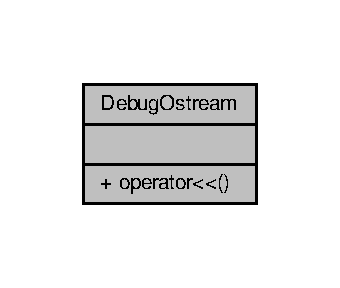
\includegraphics[width=163pt]{structDebugOstream__coll__graph}
\end{center}
\end{figure}


The documentation for this struct was generated from the following file\+:\begin{DoxyCompactItemize}
\item 
src/util.\+h\end{DoxyCompactItemize}

\hypertarget{structCode__attribute_1_1exception}{}\section{Code\+\_\+attribute\+:\+:exception Struct Reference}
\label{structCode__attribute_1_1exception}\index{Code\+\_\+attribute\+::exception@{Code\+\_\+attribute\+::exception}}


Collaboration diagram for Code\+\_\+attribute\+:\+:exception\+:\nopagebreak
\begin{figure}[H]
\begin{center}
\leavevmode
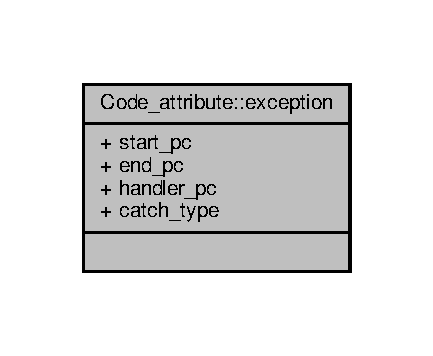
\includegraphics[width=208pt]{structCode__attribute_1_1exception__coll__graph}
\end{center}
\end{figure}


The documentation for this struct was generated from the following file\+:\begin{DoxyCompactItemize}
\item 
src/types.\+h\end{DoxyCompactItemize}

\hypertarget{structfield__info}{}\section{field\+\_\+info Struct Reference}
\label{structfield__info}\index{field\+\_\+info@{field\+\_\+info}}


Collaboration diagram for field\+\_\+info\+:
\nopagebreak
\begin{figure}[H]
\begin{center}
\leavevmode
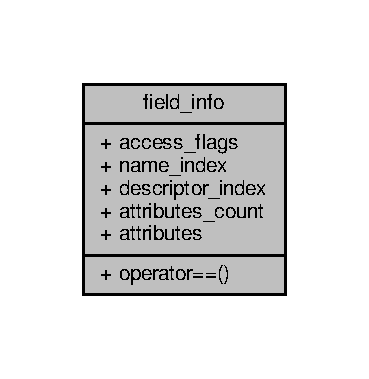
\includegraphics[width=177pt]{structfield__info__coll__graph}
\end{center}
\end{figure}


The documentation for this struct was generated from the following files\+:\begin{DoxyCompactItemize}
\item 
src/types.\+h\item 
src/types.\+cpp\end{DoxyCompactItemize}

\hypertarget{structinterface__info}{}\section{interface\+\_\+info Struct Reference}
\label{structinterface__info}\index{interface\+\_\+info@{interface\+\_\+info}}


{\ttfamily \#include $<$types.\+h$>$}



Collaboration diagram for interface\+\_\+info\+:\nopagebreak
\begin{figure}[H]
\begin{center}
\leavevmode
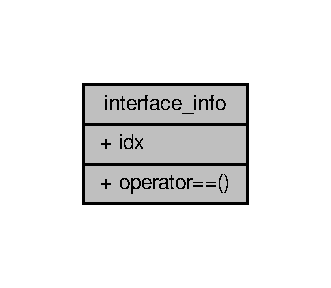
\includegraphics[width=159pt]{structinterface__info__coll__graph}
\end{center}
\end{figure}
\subsection*{Public Member Functions}
\begin{DoxyCompactItemize}
\item 
bool \hyperlink{structinterface__info_a5c19fb8052240030f2cc96876e78ed07}{operator==} (const \hyperlink{structinterface__info}{interface\+\_\+info} \&other) const
\end{DoxyCompactItemize}
\subsection*{Public Attributes}
\begin{DoxyCompactItemize}
\item 
\hyperlink{types_8h_ae676e9207f57fb921dca7366b2f59c53}{u2} \hyperlink{structinterface__info_a81fa7682cd2b314e79cb6ace44fda442}{idx}
\end{DoxyCompactItemize}


\subsection{Detailed Description}
Each value in the interfaces array must be a valid index into the constant\+\_\+pool table. The constant\+\_\+pool entry at each value of interfaces\mbox{[}i\mbox{]}, where 0 $<$= i $<$ interfaces\+\_\+count, must be tagged with \hyperlink{structcp__info_acdef8472ed83e12e3a87bca8d6001f69adf4763ef84792f4fab0a07fcb179de22}{cp\+\_\+info\+::\+Tag\+::\+C\+O\+N\+S\+T\+A\+N\+T\+\_\+\+Class} representing an interface that is a direct superinterface of this class or interface type, in the left-\/to-\/right order given in the source for the type. 

\subsection{Member Function Documentation}
\mbox{\Hypertarget{structinterface__info_a5c19fb8052240030f2cc96876e78ed07}\label{structinterface__info_a5c19fb8052240030f2cc96876e78ed07}} 
\index{interface\+\_\+info@{interface\+\_\+info}!operator==@{operator==}}
\index{operator==@{operator==}!interface\+\_\+info@{interface\+\_\+info}}
\subsubsection{\texorpdfstring{operator==()}{operator==()}}
{\footnotesize\ttfamily bool interface\+\_\+info\+::operator== (\begin{DoxyParamCaption}\item[{const \hyperlink{structinterface__info}{interface\+\_\+info} \&}]{other }\end{DoxyParamCaption}) const}



\subsection{Member Data Documentation}
\mbox{\Hypertarget{structinterface__info_a81fa7682cd2b314e79cb6ace44fda442}\label{structinterface__info_a81fa7682cd2b314e79cb6ace44fda442}} 
\index{interface\+\_\+info@{interface\+\_\+info}!idx@{idx}}
\index{idx@{idx}!interface\+\_\+info@{interface\+\_\+info}}
\subsubsection{\texorpdfstring{idx}{idx}}
{\footnotesize\ttfamily \hyperlink{types_8h_ae676e9207f57fb921dca7366b2f59c53}{u2} interface\+\_\+info\+::idx}



The documentation for this struct was generated from the following files\+:\begin{DoxyCompactItemize}
\item 
src/\hyperlink{types_8h}{types.\+h}\item 
src/\hyperlink{types_8cpp}{types.\+cpp}\end{DoxyCompactItemize}

\hypertarget{classMethod}{}\section{Method Class Reference}
\label{classMethod}\index{Method@{Method}}


This represents a view into a method reference of a class file.  




{\ttfamily \#include $<$method.\+h$>$}



Collaboration diagram for Method\+:\nopagebreak
\begin{figure}[H]
\begin{center}
\leavevmode
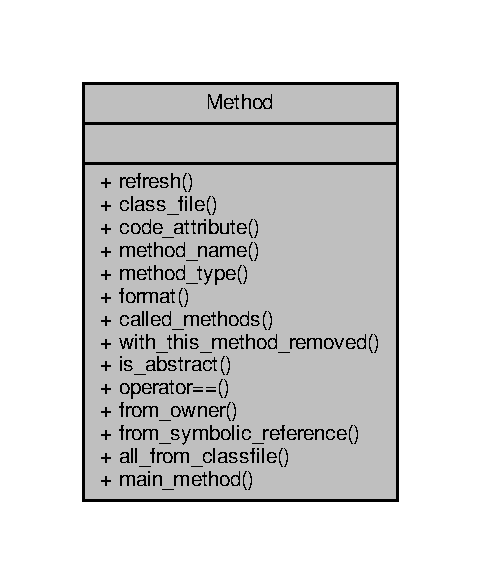
\includegraphics[width=231pt]{classMethod__coll__graph}
\end{center}
\end{figure}
\subsection*{Public Types}
\begin{DoxyCompactItemize}
\item 
\mbox{\Hypertarget{classMethod_a142a92c7e2c79cbbedb7fd08a8a8e1ad}\label{classMethod_a142a92c7e2c79cbbedb7fd08a8a8e1ad}} 
enum \hyperlink{classMethod_a142a92c7e2c79cbbedb7fd08a8a8e1ad}{F\+L\+A\+GS} \begin{DoxyCompactList}\small\item\em Enum of the access flags for a given method. \end{DoxyCompactList}
\end{DoxyCompactItemize}
\subsection*{Public Member Functions}
\begin{DoxyCompactItemize}
\item 
\hyperlink{classMethod}{Method} \hyperlink{classMethod_ac6a47d5797a62c5ffbb39df54ff7171d}{refresh} (const Class\+File \&new\+\_\+file) const
\item 
\mbox{\Hypertarget{classMethod_ac6eecb9ebb1eb23098c8556752353a81}\label{classMethod_ac6eecb9ebb1eb23098c8556752353a81}} 
const Class\+File \& \hyperlink{classMethod_ac6eecb9ebb1eb23098c8556752353a81}{class\+\_\+file} () const
\begin{DoxyCompactList}\small\item\em Returns the class file where this class belongs. \end{DoxyCompactList}\item 
std\+::optional$<$ \hyperlink{structCode__attribute}{Code\+\_\+attribute} $>$ \hyperlink{classMethod_af92b40aa1a81df3a6827d688adc005bf}{code\+\_\+attribute} () const
\item 
\mbox{\Hypertarget{classMethod_ab0855cbda89f070acc27ebff025ffd15}\label{classMethod_ab0855cbda89f070acc27ebff025ffd15}} 
std\+::string \hyperlink{classMethod_ab0855cbda89f070acc27ebff025ffd15}{method\+\_\+name} () const
\begin{DoxyCompactList}\small\item\em Returns the name of this method. \end{DoxyCompactList}\item 
\mbox{\Hypertarget{classMethod_a86015f24da420dc7502bdac6138a4a47}\label{classMethod_a86015f24da420dc7502bdac6138a4a47}} 
std\+::string \hyperlink{classMethod_a86015f24da420dc7502bdac6138a4a47}{method\+\_\+type} () const
\begin{DoxyCompactList}\small\item\em Returns the type of this method. \end{DoxyCompactList}\item 
std\+::string \hyperlink{classMethod_a3f6d55a368a1e2727bea0799c3cdc0f6}{format} () const
\item 
\mbox{\Hypertarget{classMethod_a378e12e19cf0c8f21bfc13071382d15e}\label{classMethod_a378e12e19cf0c8f21bfc13071382d15e}} 
std\+::vector$<$ \hyperlink{classMethod}{Method} $>$ \hyperlink{classMethod_a378e12e19cf0c8f21bfc13071382d15e}{called\+\_\+methods} () const
\begin{DoxyCompactList}\small\item\em Returns all the methods that {\itshape this} method calls directly. \end{DoxyCompactList}\item 
Class\+File \hyperlink{classMethod_a52e769352ce657232db3a1b936e930b1}{with\+\_\+this\+\_\+method\+\_\+removed} () const
\item 
\mbox{\Hypertarget{classMethod_a6dfb75c6faf8961c6e04a86eca6e97e8}\label{classMethod_a6dfb75c6faf8961c6e04a86eca6e97e8}} 
bool \hyperlink{classMethod_a6dfb75c6faf8961c6e04a86eca6e97e8}{is\+\_\+abstract} () const
\begin{DoxyCompactList}\small\item\em Returns whether this method is abstract. \end{DoxyCompactList}\item 
bool \hyperlink{classMethod_afa02f09f3037782d08463433465181b6}{operator==} (const \hyperlink{classMethod}{Method} \&o) const
\end{DoxyCompactItemize}
\subsection*{Static Public Member Functions}
\begin{DoxyCompactItemize}
\item 
static \hyperlink{classMethod}{Method} \hyperlink{classMethod_ad977afdb14569e1108c6b6849fe0b007}{from\+\_\+owner} (const Class\+File \&file, int index, \hyperlink{structmethod__info}{method\+\_\+info} info)
\item 
static std\+::optional$<$ \hyperlink{classMethod}{Method} $>$ \hyperlink{classMethod_adddc54ce699dfb1ba305595507085a29}{from\+\_\+symbolic\+\_\+reference} (const Class\+File \&file, int cp\+\_\+index, \hyperlink{structcp__info}{cp\+\_\+info} info)
\item 
\mbox{\Hypertarget{classMethod_a7b631e75e7438bb79c285b1bc6a712ab}\label{classMethod_a7b631e75e7438bb79c285b1bc6a712ab}} 
static std\+::vector$<$ \hyperlink{classMethod}{Method} $>$ \hyperlink{classMethod_a7b631e75e7438bb79c285b1bc6a712ab}{all\+\_\+from\+\_\+classfile} (const Class\+File \&file)
\begin{DoxyCompactList}\small\item\em Returns all the methods referenced in {\ttfamily file}. \end{DoxyCompactList}\item 
\mbox{\Hypertarget{classMethod_a74801df628f1be6e2c616cf5feb328b1}\label{classMethod_a74801df628f1be6e2c616cf5feb328b1}} 
static std\+::optional$<$ \hyperlink{classMethod}{Method} $>$ \hyperlink{classMethod_a74801df628f1be6e2c616cf5feb328b1}{main\+\_\+method} (const Class\+File \&file)
\begin{DoxyCompactList}\small\item\em Tries to retrieve the main method of {\ttfamily file}. \end{DoxyCompactList}\end{DoxyCompactItemize}


\subsection{Detailed Description}
This represents a view into a method reference of a class file. 

\subsection{Member Function Documentation}
\mbox{\Hypertarget{classMethod_af92b40aa1a81df3a6827d688adc005bf}\label{classMethod_af92b40aa1a81df3a6827d688adc005bf}} 
\index{Method@{Method}!code\+\_\+attribute@{code\+\_\+attribute}}
\index{code\+\_\+attribute@{code\+\_\+attribute}!Method@{Method}}
\subsubsection{\texorpdfstring{code\+\_\+attribute()}{code\_attribute()}}
{\footnotesize\ttfamily std\+::optional$<$ \hyperlink{structCode__attribute}{Code\+\_\+attribute} $>$ Method\+::code\+\_\+attribute (\begin{DoxyParamCaption}{ }\end{DoxyParamCaption}) const}

Returns the code attribute struct corresponding to this method. If this method is abstract, then it does not contain any code. Here is the call graph for this function\+:\nopagebreak
\begin{figure}[H]
\begin{center}
\leavevmode
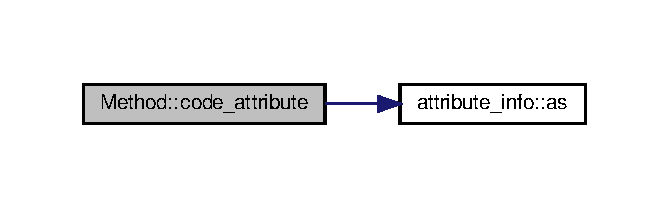
\includegraphics[width=321pt]{classMethod_af92b40aa1a81df3a6827d688adc005bf_cgraph}
\end{center}
\end{figure}
\mbox{\Hypertarget{classMethod_a3f6d55a368a1e2727bea0799c3cdc0f6}\label{classMethod_a3f6d55a368a1e2727bea0799c3cdc0f6}} 
\index{Method@{Method}!format@{format}}
\index{format@{format}!Method@{Method}}
\subsubsection{\texorpdfstring{format()}{format()}}
{\footnotesize\ttfamily std\+::string Method\+::format (\begin{DoxyParamCaption}{ }\end{DoxyParamCaption}) const}

Format this method for human view with the class name, method name and method type. This can be used for method comparison if the methods belong to updated class files, as the string is independent of the method\textquotesingle{}s index. \mbox{\Hypertarget{classMethod_ad977afdb14569e1108c6b6849fe0b007}\label{classMethod_ad977afdb14569e1108c6b6849fe0b007}} 
\index{Method@{Method}!from\+\_\+owner@{from\+\_\+owner}}
\index{from\+\_\+owner@{from\+\_\+owner}!Method@{Method}}
\subsubsection{\texorpdfstring{from\+\_\+owner()}{from\_owner()}}
{\footnotesize\ttfamily \hyperlink{classMethod}{Method} Method\+::from\+\_\+owner (\begin{DoxyParamCaption}\item[{const Class\+File \&}]{file,  }\item[{int}]{index,  }\item[{\hyperlink{structmethod__info}{method\+\_\+info}}]{info }\end{DoxyParamCaption})\hspace{0.3cm}{\ttfamily [static]}}

Static constructors for a method struct. They require a third redundant parameter in order to assert that they are being called correctly.

Constructs the method from the Class\+File which owns this method, and the method info.

This should be called as such\+: \hyperlink{classMethod_ad977afdb14569e1108c6b6849fe0b007}{Method\+::from\+\_\+owner}(file, index, file.\+methods\mbox{[}index\mbox{]}). \mbox{\Hypertarget{classMethod_adddc54ce699dfb1ba305595507085a29}\label{classMethod_adddc54ce699dfb1ba305595507085a29}} 
\index{Method@{Method}!from\+\_\+symbolic\+\_\+reference@{from\+\_\+symbolic\+\_\+reference}}
\index{from\+\_\+symbolic\+\_\+reference@{from\+\_\+symbolic\+\_\+reference}!Method@{Method}}
\subsubsection{\texorpdfstring{from\+\_\+symbolic\+\_\+reference()}{from\_symbolic\_reference()}}
{\footnotesize\ttfamily std\+::optional$<$ \hyperlink{classMethod}{Method} $>$ Method\+::from\+\_\+symbolic\+\_\+reference (\begin{DoxyParamCaption}\item[{const Class\+File \&}]{file,  }\item[{int}]{cp\+\_\+index,  }\item[{\hyperlink{structcp__info}{cp\+\_\+info}}]{info }\end{DoxyParamCaption})\hspace{0.3cm}{\ttfamily [static]}}

This method is referenced by {\ttfamily file} at the index {\ttfamily cp\+\_\+index} of the constant pool. We first have to resolve the reference, and then instantiate the method. This returns an optional, instead of the method itself, because the refernce may point to a library method, which we do not have access to.

This should be called as such\+: \hyperlink{classMethod_adddc54ce699dfb1ba305595507085a29}{Method\+::from\+\_\+symbolic\+\_\+reference}(file, index, file.\+constant\+\_\+pool\mbox{[}index\mbox{]}).

This method implicitly relies on the global project state, because the referenced method may not always be part of the current class. \mbox{\Hypertarget{classMethod_afa02f09f3037782d08463433465181b6}\label{classMethod_afa02f09f3037782d08463433465181b6}} 
\index{Method@{Method}!operator==@{operator==}}
\index{operator==@{operator==}!Method@{Method}}
\subsubsection{\texorpdfstring{operator==()}{operator==()}}
{\footnotesize\ttfamily bool Method\+::operator== (\begin{DoxyParamCaption}\item[{const \hyperlink{classMethod}{Method} \&}]{o }\end{DoxyParamCaption}) const}

This compares based based on class file and index, not on actual value. In other words, updating the class file will cause methods to compre unequal. Here is the call graph for this function\+:\nopagebreak
\begin{figure}[H]
\begin{center}
\leavevmode
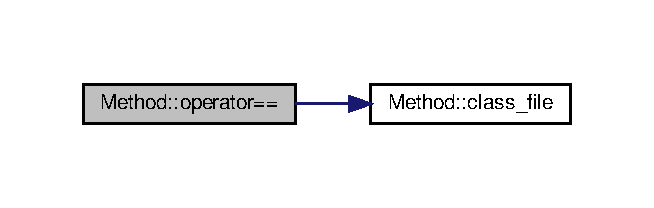
\includegraphics[width=314pt]{classMethod_afa02f09f3037782d08463433465181b6_cgraph}
\end{center}
\end{figure}
\mbox{\Hypertarget{classMethod_ac6a47d5797a62c5ffbb39df54ff7171d}\label{classMethod_ac6a47d5797a62c5ffbb39df54ff7171d}} 
\index{Method@{Method}!refresh@{refresh}}
\index{refresh@{refresh}!Method@{Method}}
\subsubsection{\texorpdfstring{refresh()}{refresh()}}
{\footnotesize\ttfamily \hyperlink{classMethod}{Method} Method\+::refresh (\begin{DoxyParamCaption}\item[{const Class\+File \&}]{new\+\_\+file }\end{DoxyParamCaption}) const}

After a class file has been changed, {\itshape this} method will still reference the old one. In order to resolve this method in the new class file, it has to search for the new index and create a new struct. Here is the call graph for this function\+:\nopagebreak
\begin{figure}[H]
\begin{center}
\leavevmode
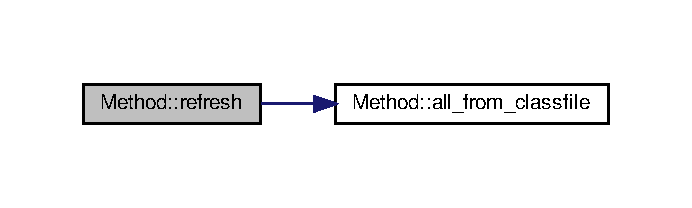
\includegraphics[width=332pt]{classMethod_ac6a47d5797a62c5ffbb39df54ff7171d_cgraph}
\end{center}
\end{figure}
\mbox{\Hypertarget{classMethod_a52e769352ce657232db3a1b936e930b1}\label{classMethod_a52e769352ce657232db3a1b936e930b1}} 
\index{Method@{Method}!with\+\_\+this\+\_\+method\+\_\+removed@{with\+\_\+this\+\_\+method\+\_\+removed}}
\index{with\+\_\+this\+\_\+method\+\_\+removed@{with\+\_\+this\+\_\+method\+\_\+removed}!Method@{Method}}
\subsubsection{\texorpdfstring{with\+\_\+this\+\_\+method\+\_\+removed()}{with\_this\_method\_removed()}}
{\footnotesize\ttfamily Class\+File Method\+::with\+\_\+this\+\_\+method\+\_\+removed (\begin{DoxyParamCaption}{ }\end{DoxyParamCaption}) const}

Removes {\itshape this} method from the original class file, returning a new one with this method removed. 

The documentation for this class was generated from the following files\+:\begin{DoxyCompactItemize}
\item 
src/method.\+h\item 
src/method.\+cpp\end{DoxyCompactItemize}

\hypertarget{structmethod__info}{}\section{method\+\_\+info Struct Reference}
\label{structmethod__info}\index{method\+\_\+info@{method\+\_\+info}}


Collaboration diagram for method\+\_\+info\+:
\nopagebreak
\begin{figure}[H]
\begin{center}
\leavevmode
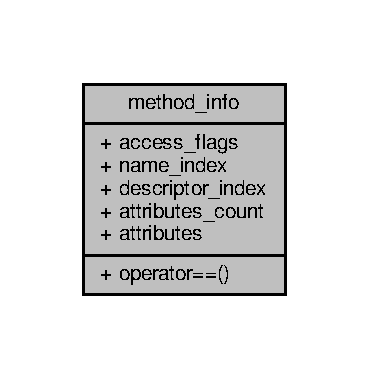
\includegraphics[width=177pt]{structmethod__info__coll__graph}
\end{center}
\end{figure}


The documentation for this struct was generated from the following files\+:\begin{DoxyCompactItemize}
\item 
src/types.\+h\item 
src/types.\+cpp\end{DoxyCompactItemize}

\hypertarget{classProject}{}\section{Project Class Reference}
\label{classProject}\index{Project@{Project}}


A \hyperlink{classProject}{Project} is a collection of class files, together with a main entry point.  




{\ttfamily \#include $<$project.\+h$>$}



Collaboration diagram for Project\+:
\nopagebreak
\begin{figure}[H]
\begin{center}
\leavevmode
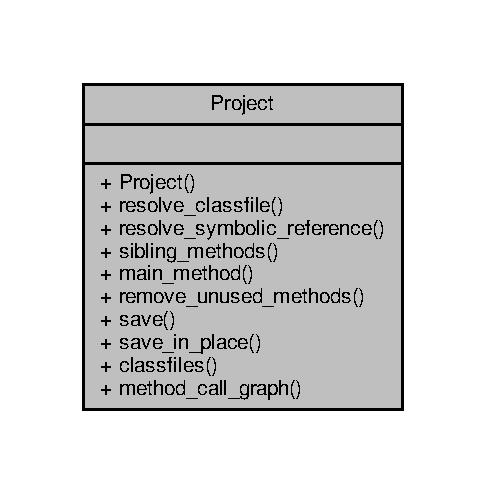
\includegraphics[width=233pt]{classProject__coll__graph}
\end{center}
\end{figure}
\subsection*{Public Member Functions}
\begin{DoxyCompactItemize}
\item 
\hyperlink{classProject_aa263ab552c113e7a9db9e90c3dac0879}{Project} (std\+::vector$<$ std\+::experimental\+::filesystem\+::path $>$ class\+\_\+files)
\item 
std\+::optional$<$ \hyperlink{classfile_8h_a00b46b60bc40e813e9fb1bb049174346}{Class\+File} $>$ \hyperlink{classProject_a2ec0981bc841bcbac0ca8072f3b960b5}{resolve\+\_\+classfile} (const std\+::string \&class\+\_\+name) const
\begin{DoxyCompactList}\small\item\em Find the appropiate class file given the name. \end{DoxyCompactList}\item 
std\+::optional$<$ \hyperlink{classMethod}{Method} $>$ \hyperlink{classProject_a2bf65efcb1e91bfe76d2faab76127c11}{resolve\+\_\+symbolic\+\_\+reference} (const std\+::string \&class\+\_\+name, const std\+::string \&method\+\_\+name, const std\+::string \&method\+\_\+type) const
\item 
std\+::vector$<$ \hyperlink{classMethod}{Method} $>$ \hyperlink{classProject_afee58125bfee1c7a1871be7805e855fa}{sibling\+\_\+methods} (const \hyperlink{classMethod}{Method} \&m) const
\item 
\hyperlink{classMethod}{Method} \hyperlink{classProject_a8122de9e7b4bc2a63e1391727c881474}{main\+\_\+method} () const
\begin{DoxyCompactList}\small\item\em Find the main entry point of the entire project. \end{DoxyCompactList}\item 
void \hyperlink{classProject_af5f35c59d1175af1cfa659a597bb6353}{remove\+\_\+unused\+\_\+methods} ()
\item 
void \hyperlink{classProject_aff5e62e0e0e3e8c7123a7dd6ae51cb3f}{save} (std\+::experimental\+::filesystem\+::path path) const
\begin{DoxyCompactList}\small\item\em Save all of the class files in the given location. \end{DoxyCompactList}\item 
void \hyperlink{classProject_aecff214fd8b3fc5e855ec925ebe93f59}{save\+\_\+in\+\_\+place} (std\+::vector$<$ std\+::experimental\+::filesystem\+::path $>$ filenames) const
\begin{DoxyCompactList}\small\item\em Save all of the files in-\/place. \end{DoxyCompactList}\item 
std\+::vector$<$ \hyperlink{classfile_8h_a00b46b60bc40e813e9fb1bb049174346}{Class\+File} $>$ \hyperlink{classProject_a74b0dfe1d19f11e859489922a8d277c7}{classfiles} () const
\begin{DoxyCompactList}\small\item\em Returns all of the class files. \end{DoxyCompactList}\item 
std\+::vector$<$ \hyperlink{classMethod}{Method} $>$ \hyperlink{classProject_ac4d866eaedfd1083d4736530382c7b7c}{method\+\_\+call\+\_\+graph} (const \hyperlink{classMethod}{Method} \&m) const
\end{DoxyCompactItemize}
\subsection*{Private Member Functions}
\begin{DoxyCompactItemize}
\item 
bool \hyperlink{classProject_a6ef93527bbe86e9bdfbc6d624eab0834}{class\+\_\+is\+\_\+descendant} (const \hyperlink{classfile_8h_a00b46b60bc40e813e9fb1bb049174346}{Class\+File} \&down, const \hyperlink{classfile_8h_a00b46b60bc40e813e9fb1bb049174346}{Class\+File} \&up) const
\end{DoxyCompactItemize}
\subsection*{Private Attributes}
\begin{DoxyCompactItemize}
\item 
std\+::vector$<$ \hyperlink{classfile_8h_a00b46b60bc40e813e9fb1bb049174346}{Class\+File} $>$ \hyperlink{classProject_a33de2bfb90183333d5e7c422bc5d6396}{m\+\_\+files}
\end{DoxyCompactItemize}


\subsection{Detailed Description}
A \hyperlink{classProject}{Project} is a collection of class files, together with a main entry point. 

\subsection{Constructor \& Destructor Documentation}
\mbox{\Hypertarget{classProject_aa263ab552c113e7a9db9e90c3dac0879}\label{classProject_aa263ab552c113e7a9db9e90c3dac0879}} 
\index{Project@{Project}!Project@{Project}}
\index{Project@{Project}!Project@{Project}}
\subsubsection{\texorpdfstring{Project()}{Project()}}
{\footnotesize\ttfamily Project\+::\+Project (\begin{DoxyParamCaption}\item[{std\+::vector$<$ std\+::experimental\+::filesystem\+::path $>$}]{class\+\_\+files }\end{DoxyParamCaption})}

Here is the call graph for this function\+:
\nopagebreak
\begin{figure}[H]
\begin{center}
\leavevmode
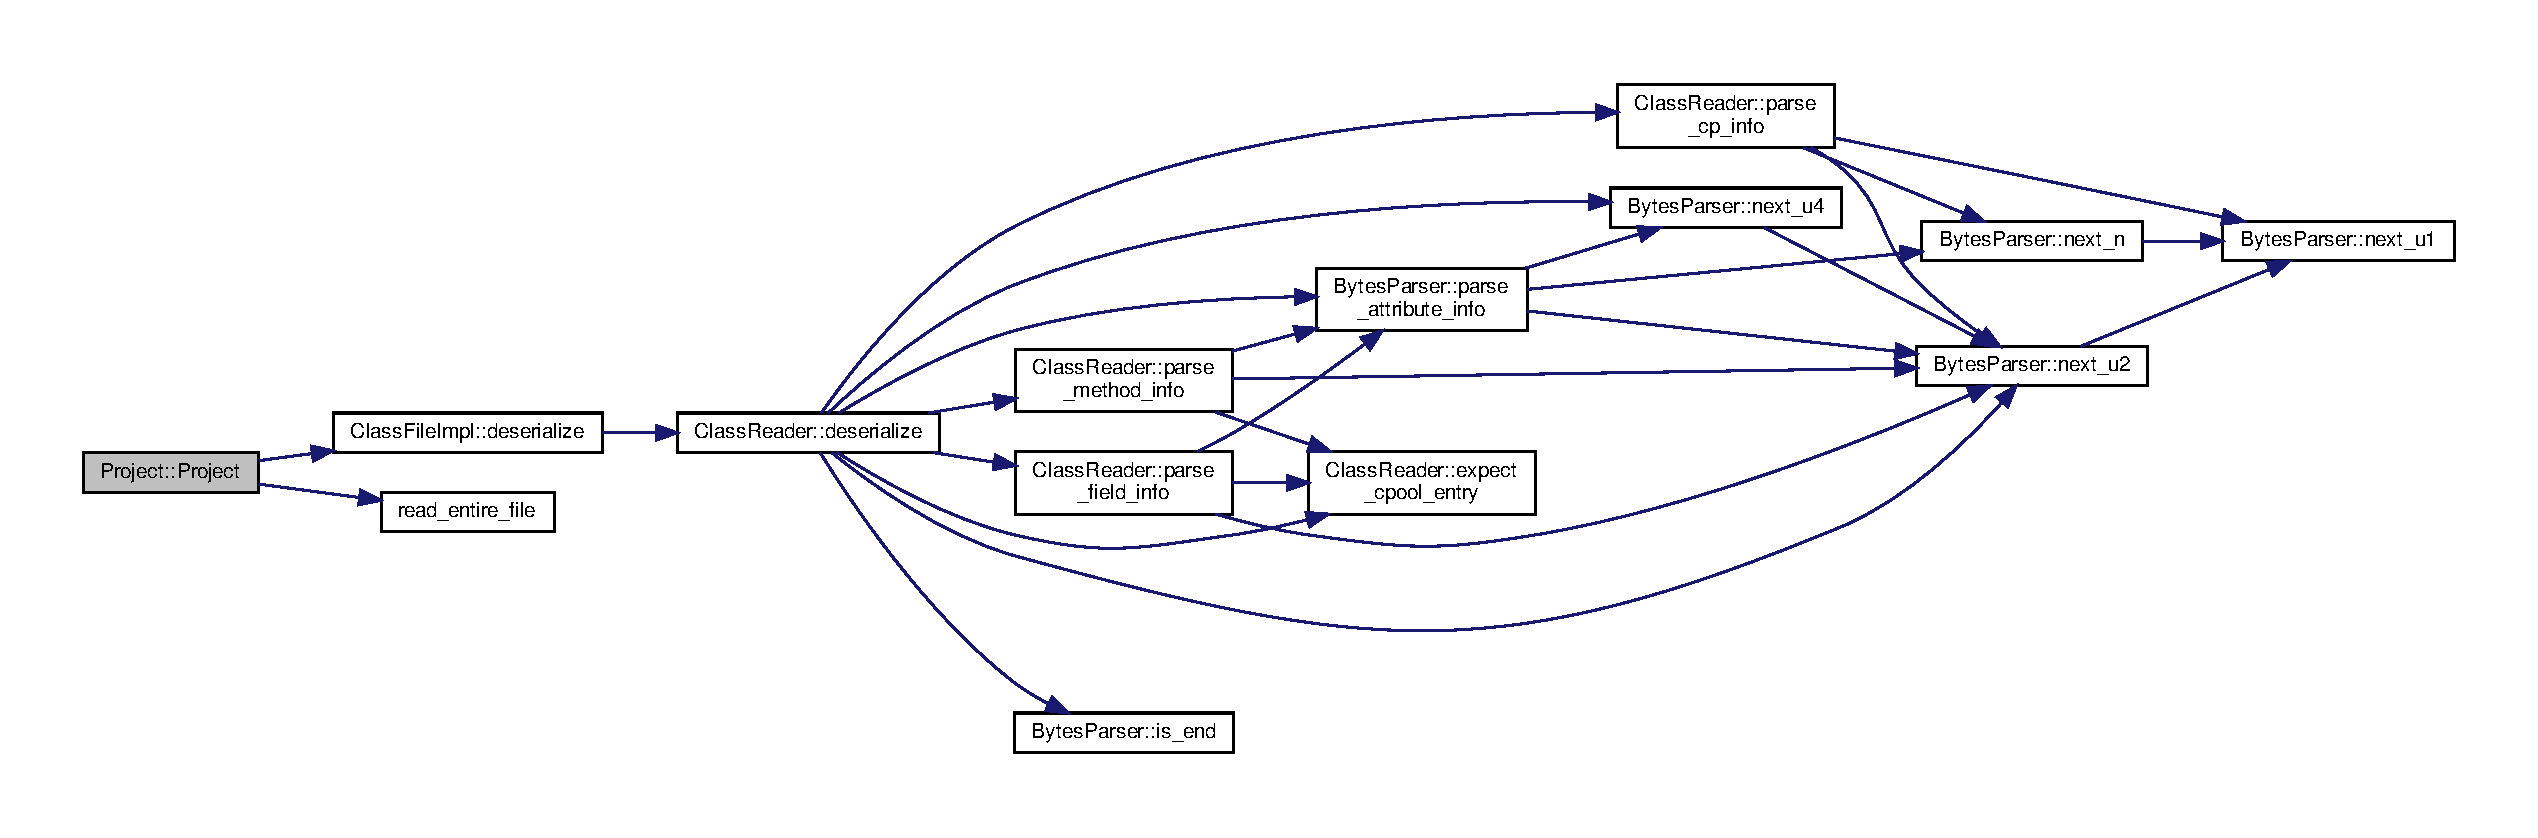
\includegraphics[width=350pt]{classProject_aa263ab552c113e7a9db9e90c3dac0879_cgraph}
\end{center}
\end{figure}


\subsection{Member Function Documentation}
\mbox{\Hypertarget{classProject_a6ef93527bbe86e9bdfbc6d624eab0834}\label{classProject_a6ef93527bbe86e9bdfbc6d624eab0834}} 
\index{Project@{Project}!class\+\_\+is\+\_\+descendant@{class\+\_\+is\+\_\+descendant}}
\index{class\+\_\+is\+\_\+descendant@{class\+\_\+is\+\_\+descendant}!Project@{Project}}
\subsubsection{\texorpdfstring{class\+\_\+is\+\_\+descendant()}{class\_is\_descendant()}}
{\footnotesize\ttfamily bool Project\+::class\+\_\+is\+\_\+descendant (\begin{DoxyParamCaption}\item[{const \hyperlink{classfile_8h_a00b46b60bc40e813e9fb1bb049174346}{Class\+File} \&}]{down,  }\item[{const \hyperlink{classfile_8h_a00b46b60bc40e813e9fb1bb049174346}{Class\+File} \&}]{up }\end{DoxyParamCaption}) const\hspace{0.3cm}{\ttfamily [private]}}

Returns whether the two classes are in some way related\+: there is a path in the directed inheritance graph from down to up. Here is the call graph for this function\+:
\nopagebreak
\begin{figure}[H]
\begin{center}
\leavevmode
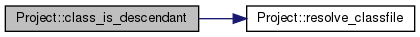
\includegraphics[width=350pt]{classProject_a6ef93527bbe86e9bdfbc6d624eab0834_cgraph}
\end{center}
\end{figure}
\mbox{\Hypertarget{classProject_a74b0dfe1d19f11e859489922a8d277c7}\label{classProject_a74b0dfe1d19f11e859489922a8d277c7}} 
\index{Project@{Project}!classfiles@{classfiles}}
\index{classfiles@{classfiles}!Project@{Project}}
\subsubsection{\texorpdfstring{classfiles()}{classfiles()}}
{\footnotesize\ttfamily std\+::vector$<$ \hyperlink{classfile_8h_a00b46b60bc40e813e9fb1bb049174346}{Class\+File} $>$ Project\+::classfiles (\begin{DoxyParamCaption}{ }\end{DoxyParamCaption}) const}



Returns all of the class files. 

\mbox{\Hypertarget{classProject_a8122de9e7b4bc2a63e1391727c881474}\label{classProject_a8122de9e7b4bc2a63e1391727c881474}} 
\index{Project@{Project}!main\+\_\+method@{main\+\_\+method}}
\index{main\+\_\+method@{main\+\_\+method}!Project@{Project}}
\subsubsection{\texorpdfstring{main\+\_\+method()}{main\_method()}}
{\footnotesize\ttfamily \hyperlink{classMethod}{Method} Project\+::main\+\_\+method (\begin{DoxyParamCaption}{ }\end{DoxyParamCaption}) const}



Find the main entry point of the entire project. 

Here is the call graph for this function\+:
\nopagebreak
\begin{figure}[H]
\begin{center}
\leavevmode
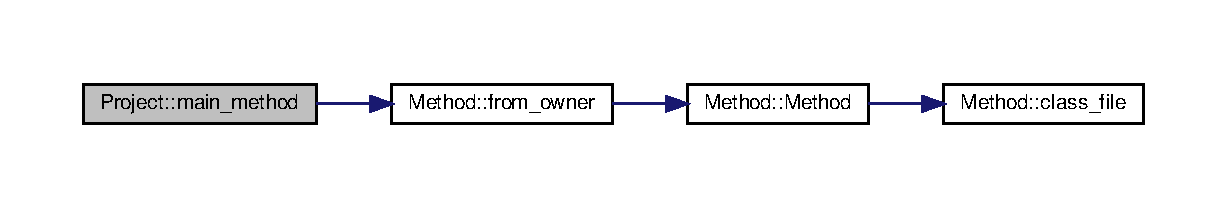
\includegraphics[width=350pt]{classProject_a8122de9e7b4bc2a63e1391727c881474_cgraph}
\end{center}
\end{figure}
\mbox{\Hypertarget{classProject_ac4d866eaedfd1083d4736530382c7b7c}\label{classProject_ac4d866eaedfd1083d4736530382c7b7c}} 
\index{Project@{Project}!method\+\_\+call\+\_\+graph@{method\+\_\+call\+\_\+graph}}
\index{method\+\_\+call\+\_\+graph@{method\+\_\+call\+\_\+graph}!Project@{Project}}
\subsubsection{\texorpdfstring{method\+\_\+call\+\_\+graph()}{method\_call\_graph()}}
{\footnotesize\ttfamily std\+::vector$<$ \hyperlink{classMethod}{Method} $>$ Project\+::method\+\_\+call\+\_\+graph (\begin{DoxyParamCaption}\item[{const \hyperlink{classMethod}{Method} \&}]{m }\end{DoxyParamCaption}) const}

Returns all of the methods which are reachable by a series of calls from the given method. Here is the call graph for this function\+:
\nopagebreak
\begin{figure}[H]
\begin{center}
\leavevmode
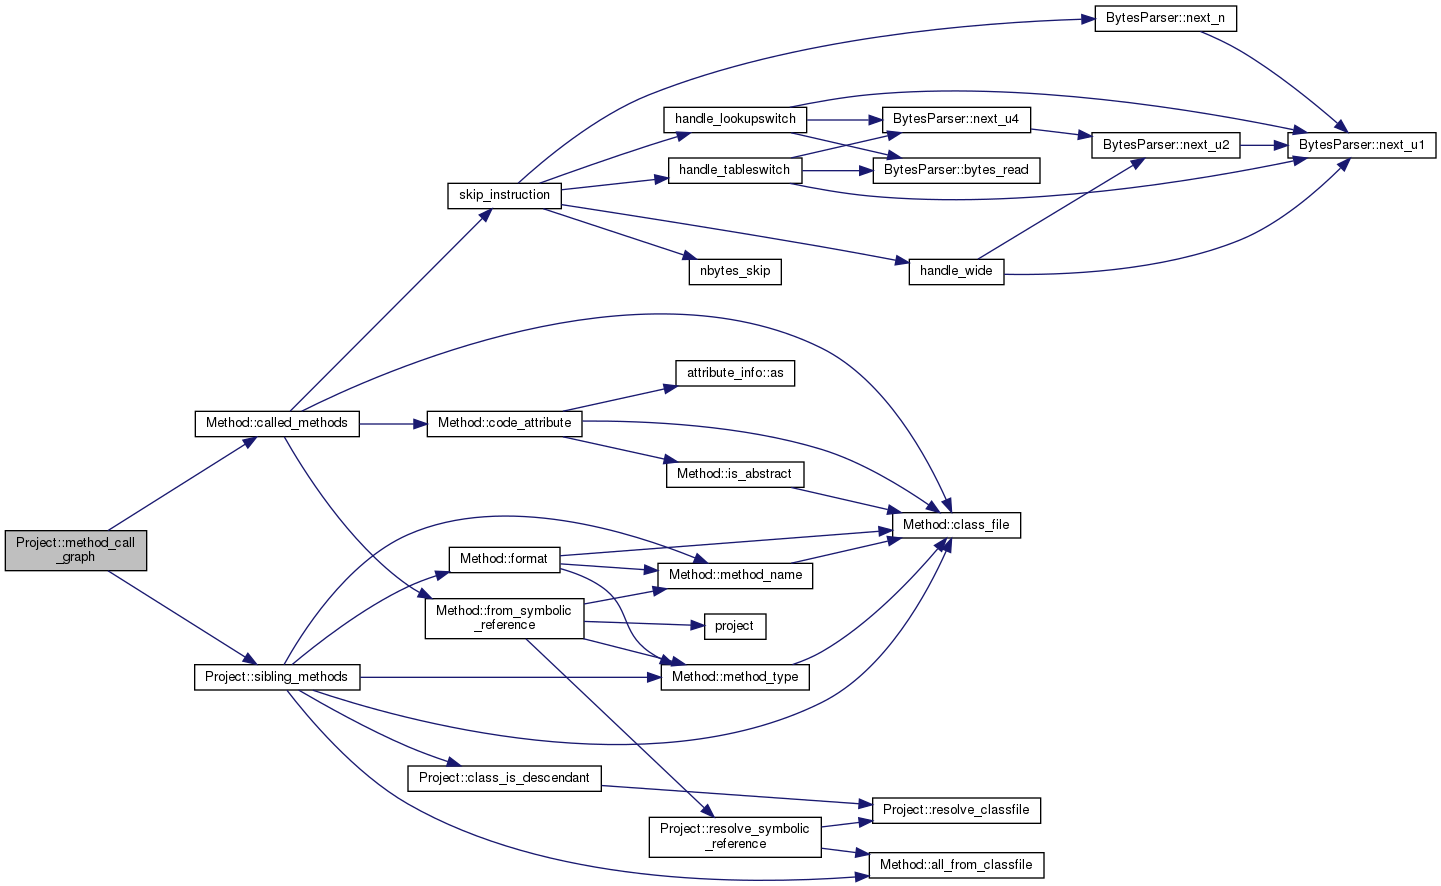
\includegraphics[width=350pt]{classProject_ac4d866eaedfd1083d4736530382c7b7c_cgraph}
\end{center}
\end{figure}
\mbox{\Hypertarget{classProject_af5f35c59d1175af1cfa659a597bb6353}\label{classProject_af5f35c59d1175af1cfa659a597bb6353}} 
\index{Project@{Project}!remove\+\_\+unused\+\_\+methods@{remove\+\_\+unused\+\_\+methods}}
\index{remove\+\_\+unused\+\_\+methods@{remove\+\_\+unused\+\_\+methods}!Project@{Project}}
\subsubsection{\texorpdfstring{remove\+\_\+unused\+\_\+methods()}{remove\_unused\_methods()}}
{\footnotesize\ttfamily void Project\+::remove\+\_\+unused\+\_\+methods (\begin{DoxyParamCaption}{ }\end{DoxyParamCaption})}

This is for now not purely functional, due to the global resolution of method references via the {\ttfamily \hyperlink{project_8cpp_a3c33c839f231786a482d8b5a76c269d3}{project()}} function.

As Class\+Files are actively modified for each removed method, all references needs need to be re-\/resolved after every deletion, because they are reindexed. Due to the way external references work (class A references a method of class B), based on name and type, it is only necessary to update the methods from within the modified Class\+File. Here is the call graph for this function\+:
\nopagebreak
\begin{figure}[H]
\begin{center}
\leavevmode
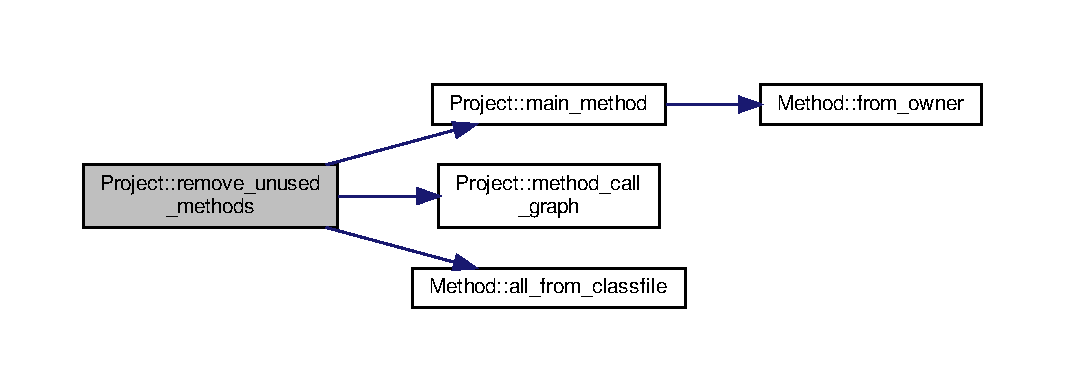
\includegraphics[width=350pt]{classProject_af5f35c59d1175af1cfa659a597bb6353_cgraph}
\end{center}
\end{figure}
\mbox{\Hypertarget{classProject_a2ec0981bc841bcbac0ca8072f3b960b5}\label{classProject_a2ec0981bc841bcbac0ca8072f3b960b5}} 
\index{Project@{Project}!resolve\+\_\+classfile@{resolve\+\_\+classfile}}
\index{resolve\+\_\+classfile@{resolve\+\_\+classfile}!Project@{Project}}
\subsubsection{\texorpdfstring{resolve\+\_\+classfile()}{resolve\_classfile()}}
{\footnotesize\ttfamily std\+::optional$<$ \hyperlink{classfile_8h_a00b46b60bc40e813e9fb1bb049174346}{Class\+File} $>$ Project\+::resolve\+\_\+classfile (\begin{DoxyParamCaption}\item[{const std\+::string \&}]{class\+\_\+name }\end{DoxyParamCaption}) const}



Find the appropiate class file given the name. 

\mbox{\Hypertarget{classProject_a2bf65efcb1e91bfe76d2faab76127c11}\label{classProject_a2bf65efcb1e91bfe76d2faab76127c11}} 
\index{Project@{Project}!resolve\+\_\+symbolic\+\_\+reference@{resolve\+\_\+symbolic\+\_\+reference}}
\index{resolve\+\_\+symbolic\+\_\+reference@{resolve\+\_\+symbolic\+\_\+reference}!Project@{Project}}
\subsubsection{\texorpdfstring{resolve\+\_\+symbolic\+\_\+reference()}{resolve\_symbolic\_reference()}}
{\footnotesize\ttfamily std\+::optional$<$ \hyperlink{classMethod}{Method} $>$ Project\+::resolve\+\_\+symbolic\+\_\+reference (\begin{DoxyParamCaption}\item[{const std\+::string \&}]{class\+\_\+name,  }\item[{const std\+::string \&}]{method\+\_\+name,  }\item[{const std\+::string \&}]{method\+\_\+type }\end{DoxyParamCaption}) const}

Here is the call graph for this function\+:
\nopagebreak
\begin{figure}[H]
\begin{center}
\leavevmode
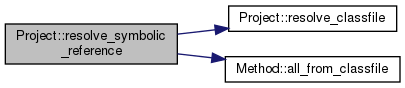
\includegraphics[width=350pt]{classProject_a2bf65efcb1e91bfe76d2faab76127c11_cgraph}
\end{center}
\end{figure}
\mbox{\Hypertarget{classProject_aff5e62e0e0e3e8c7123a7dd6ae51cb3f}\label{classProject_aff5e62e0e0e3e8c7123a7dd6ae51cb3f}} 
\index{Project@{Project}!save@{save}}
\index{save@{save}!Project@{Project}}
\subsubsection{\texorpdfstring{save()}{save()}}
{\footnotesize\ttfamily void Project\+::save (\begin{DoxyParamCaption}\item[{std\+::experimental\+::filesystem\+::path}]{path }\end{DoxyParamCaption}) const}



Save all of the class files in the given location. 

Here is the call graph for this function\+:
\nopagebreak
\begin{figure}[H]
\begin{center}
\leavevmode
\includegraphics[width=300pt]{classProject_aff5e62e0e0e3e8c7123a7dd6ae51cb3f_cgraph}
\end{center}
\end{figure}
\mbox{\Hypertarget{classProject_aecff214fd8b3fc5e855ec925ebe93f59}\label{classProject_aecff214fd8b3fc5e855ec925ebe93f59}} 
\index{Project@{Project}!save\+\_\+in\+\_\+place@{save\+\_\+in\+\_\+place}}
\index{save\+\_\+in\+\_\+place@{save\+\_\+in\+\_\+place}!Project@{Project}}
\subsubsection{\texorpdfstring{save\+\_\+in\+\_\+place()}{save\_in\_place()}}
{\footnotesize\ttfamily void Project\+::save\+\_\+in\+\_\+place (\begin{DoxyParamCaption}\item[{std\+::vector$<$ std\+::experimental\+::filesystem\+::path $>$}]{filenames }\end{DoxyParamCaption}) const}



Save all of the files in-\/place. 

Here is the call graph for this function\+:
\nopagebreak
\begin{figure}[H]
\begin{center}
\leavevmode
\includegraphics[width=342pt]{classProject_aecff214fd8b3fc5e855ec925ebe93f59_cgraph}
\end{center}
\end{figure}
\mbox{\Hypertarget{classProject_afee58125bfee1c7a1871be7805e855fa}\label{classProject_afee58125bfee1c7a1871be7805e855fa}} 
\index{Project@{Project}!sibling\+\_\+methods@{sibling\+\_\+methods}}
\index{sibling\+\_\+methods@{sibling\+\_\+methods}!Project@{Project}}
\subsubsection{\texorpdfstring{sibling\+\_\+methods()}{sibling\_methods()}}
{\footnotesize\ttfamily std\+::vector$<$ \hyperlink{classMethod}{Method} $>$ Project\+::sibling\+\_\+methods (\begin{DoxyParamCaption}\item[{const \hyperlink{classMethod}{Method} \&}]{m }\end{DoxyParamCaption}) const}

Returns all of the methods which have the same name and type as {\ttfamily m}, and belong to related classes.

For instance, a method of a descendant in the inheritance chart, because it might be that that method is called due to polymorphism. Here is the call graph for this function\+:
\nopagebreak
\begin{figure}[H]
\begin{center}
\leavevmode
\includegraphics[width=350pt]{classProject_afee58125bfee1c7a1871be7805e855fa_cgraph}
\end{center}
\end{figure}


\subsection{Member Data Documentation}
\mbox{\Hypertarget{classProject_a33de2bfb90183333d5e7c422bc5d6396}\label{classProject_a33de2bfb90183333d5e7c422bc5d6396}} 
\index{Project@{Project}!m\+\_\+files@{m\+\_\+files}}
\index{m\+\_\+files@{m\+\_\+files}!Project@{Project}}
\subsubsection{\texorpdfstring{m\+\_\+files}{m\_files}}
{\footnotesize\ttfamily std\+::vector$<$\hyperlink{classfile_8h_a00b46b60bc40e813e9fb1bb049174346}{Class\+File}$>$ Project\+::m\+\_\+files\hspace{0.3cm}{\ttfamily [private]}}



The documentation for this class was generated from the following files\+:\begin{DoxyCompactItemize}
\item 
src/\hyperlink{project_8h}{project.\+h}\item 
src/\hyperlink{project_8cpp}{project.\+cpp}\end{DoxyCompactItemize}

%--- End generated contents ---

% Index
\backmatter
\newpage
\phantomsection
\clearemptydoublepage
\addcontentsline{toc}{chapter}{Index}
\printindex

\end{document}
